\chapter{Knowledge-Based System Introduction into a Deep Learning Environment}\label{chap:kbsintegrationdl}

%Motivaciones de esto: Incrementar capacidad de generalización, reducir número de recursos, aumento de la interpretabilidad del modelo. Restricciones de esto: 
This chapter\footnote{The content of this chapter is based on the work: Amador-Domínguez, E., Serrano, E., Manrique, D., Hohenecker, P., and Lukasiewicz, T. (2021). An ontology-based deep learning approach for triple classification with out-of-knowledge-base entities. Information Sciences, 564, 85–102. doi:10.1016/j.ins.2021.02.018} focuses the first of the integrations contemplated in this thesis: the insertion of knowledge-based systems in deep learning models. Section \ref{4_sec:methodology_kbs_intro_dl} outlines the specific method parameters of this integration, along with the relations between them. This design is then materialized into a hybrid proposal for KGC. KGC is one of the main fields of application of neurosymbolic approaches, as it provides a propitious scenario where both symbolic and subsymbolic approaches are suitable. This chapter presents a semantic-based initialization approach, which can be combined with any KGE model, subsequently generating a hybrid approach. Section \ref{4_sec:ontointro_kgc} outlines the motivation and overview of the proposed initialization, presented Section \ref{4_sec:semantic_initialization}. Section \ref{4_sec:experiments} presents the different experiments conducted to validate the proposal, as well as the achieved results, which are discussed in Section \ref{4_sec:results}. Section \ref{4_sec:method_assessment} frames the presented use case in the context of the general design method, providing insights on the specific parameter values. Section \ref{4_sec:summary} summarizes the content of the chapter. 

\begin{figure}[t]
    \centering
    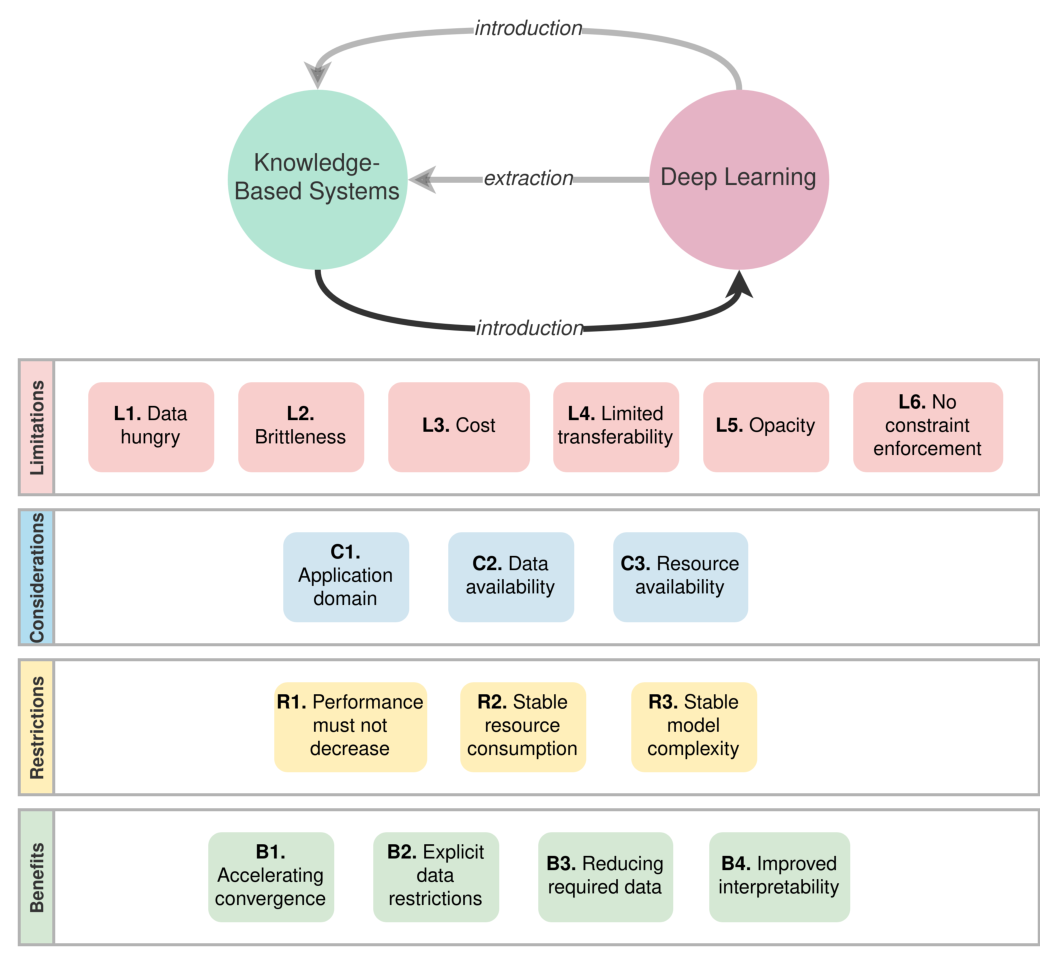
\includegraphics[width=\linewidth]{4_kbsintegrationdl/figures/overview_kbs_dl_intro.eps}
    \caption{Overview on the Insertion of Knowledge-Based Systems in Deep Learning.}
    \label{fig:overview_kbs_dl_intro}
\end{figure}

%%%LA MOVIDA DE LA SENSIA EN ESTA VERTIENTE CONCRETA
\section{Knowledge-Based System Insertion in Deep Learning Models} \label{4_sec:methodology_kbs_intro_dl}
This Section presents the design parameters for KBS insertion into DL models. In this scenario, the DL model plays the primary role, while the KBS plays the secondary role. Figure \ref{fig:overview_kbs_dl_intro} outlines the specific methodological parameters for this integration, which are defined as follows.

\paragraph{Limitations}
\begin{enumerate} [start=1,label={\bfseries L\arabic*.}]
    \item \label{kbsintrodl_L_data_hungry} \textbf{Data hungry.} This is one of the most concerning issues regarding DL. While DL is capable of achieving a better abstraction and generalization capacity than its symbolic counterpart, the final performance is highly linked to both the quality and the quantity of the data. Large, balanced, and representative training sets are required for the DL model to learn accurate patterns about the data. This limitation implies that the final performance of the model is directly bounded to its training data, thus not being a trusty indicator on the aptness of the model. 
    
    \item \label{kbsintrodl_L_brittleness} \textbf{Brittleness.} DL models infer abstract reasoning patterns from the training data. These patterns, however, may not be robust enough to correctly deal with noise. Adversarial attacks can cause DL models to fail. Therefore, even if a given DL produces an output $Y$ for a given input $X$, it can not be ensured that for a slightly corrupted version $X'$ of the input will lead to the same outcome.
    
    \item \label{kbsintrodl_L_cost} \textbf{Cost.} Training a DL model requires an elevated computational cost. While GPUs and TPUs have greatly alleviated this issue, the disparity on the availability of computational resources is a significant drawback of DL models. Not only the training time varies greatly across different infrastructures for the same implementation, but a given DL model may be incapable of training or executing if the available resources are insufficient. Maintaining computational cost at reasonable limits should therefore be prioritized.  
    
    \item \label{kbsintrodl_L_transfer} \textbf{Limited transferability.} Reusability is one of the most prominent features of DL models. Transfer learning reduces the need to retrain a given architecture from scratch to fit a new dataset or solve a new task. However, a model $M$ may achieve a remarkable performance on a given task $t$, but this performance may not  hold for a different task $t'$, even if they are fairly similar. Additionally, if a model $M'$ is trained using $M$ as a base, it can not be ascertain whether the performance of the newly trained model will be similar to the baseline.
    
    \item \label{kbsintrodl_L_opacity} \textbf{Opacity.} One of the main concerns regarding DL models is their limited explainability. DL models often provide better results than KBS on multiple tasks, but their usage is often hindered due to the impossibility to provide human-understandable insights on why a certain output is obtained.
    
    \item \label{kbsintrodl_L_constraint} \textbf{No constraint enforcement.} DL models infer patterns from a set of training samples. However, these patterns may not truthfully represent the data, as noisy or unbalanced data may negatively impact the learning process. The patterns learned by a DL model can then be inconsistent, and may not be able to properly generalize from unseen data.
    \end{enumerate}
\paragraph{Considerations}
\begin{enumerate} [start=1,label={\bfseries C\arabic*.}]
    \item \label{kbsintrodl_C_domain} \textbf{Application domain.} Table \ref{tab:sensors_reasoning} showcased an existing bias in the employed reasoning models according to their application. Complex and opaque approaches were selected in domains where their worst-case scenario impact was low (i.e. housing), while fully expressive and interpretable models were considerably favoured in human-dominated areas (i.e, healthcare). Therefore, in this scenario where the DL model is the primary, it must be studied whether the application domain strictly requires from human understandability. Even though the introduction of KBS into DL models may reduce its opacity, it may not be sufficient to fully comprehend the inference process of the model. 
    
    \item  \label{kbsintrodl_C_data} \textbf{Data availability.} As stated in \ref{kbsintrodl_L_data_hungry}, data availability is one of the main bottlenecks of DL models. This issue may be alleviated by the introduction of a KBS model. In those scenarios where the KBS model is already trained, data availability may not be an issue. However, if the KBS model needs to be trained before being integrated within the DL model, there must exists valid data to build the KBS model. Data availability for KBS model training must then be ensured beforehand.
    
    \item  \label{kbsintrodl_C_resource} \textbf{Resource availability.} This consideration is directly related to \ref{kbsintrodl_L_cost} (cost). KBS models have a much reduced computational cost in comparison to DL models. However, even if small, they still carry a computational cost that is added to the baseline cost of the DL model which should be noted. The cost of introducing the KBS model should never exceed the cost of the primary DL model.
    
\end{enumerate}
\paragraph{Restrictions}
\begin{enumerate} [start=1,label={\bfseries R\arabic*.}]
    \item \label{kbsintrodl_R_performance} \textbf{Performance must not decrease.} One of the fundamental strengths of DL models is that they provide remarkable performances on a wide variety of tasks. The introduction of a KBS model must never negatively impact the model performance, as this is a pivotal element that should therefore be preserved. While there may not be a remarkable improvement in the final metrics, for example, the correct prediction of outliers, which may represent a very small fraction of the data, the performance should, at least, remain stable.
    
    \item \label{kbsintrodl_R_resource} \textbf{Stable resource consumption.} The introduction of an additional model subsequently carries an additional cost. As noted in \ref{kbsintrodl_C_resource} (resource availability), this increment must be taken into consideration. The overall resource consumption of the model must remain within reasonable bounds (\ref{kbsintrodl_L_cost}), and the final model should be able to train and operate with the previously existing resources.
    
    \item \label{kbsintrodl_R_complexity} \textbf{Stable model complexity.} DL models are generally complex and suffer from elevated training times. Therefore, the KBS model should not add an additional complexity to the DL model. For this purpose, whenever possible, the KBS model must not be fully coupled with the DL model. Instead, it may be devised as an individual component that is actively involved in the training process of the DL model, but does not add any additional complexity to the model itself. 
    
\end{enumerate}
\paragraph{Benefits}
\begin{enumerate} [start=1,label={\bfseries B\arabic*.}]
    \item \label{kbsintrodl_B_convergence} \textbf{Accelerate convergence.} As noted in \ref{kbsintrodl_R_complexity}, DL models may suffer from elevated training times. This issue may be eased with the inclusion of a KBS, which already models knowledge about the data that the DL model may not even be capable of inferring otherwise. The introduction of this additional knowledge can not only lead to better performances, but reduce the training time as the model may converge faster to its optimal solution, reducing its computational cost (\ref{kbsintrodl_L_cost}).
    
    \item \label{kbsintrodl_B_restrictions} \textbf{Explicit data restrictions.} During training DL models internally learn restrictions and constraints about the data. As stated in \ref{kbsintrodl_L_constraint}, the implicit constraints about the data may be inconsistent, leading to errors. KBS extract explicit constraints and patterns from the data, which are then use to perform reasoning (e.g. rule-based systems, decision trees), that may not be inferred using a DL model. These restrictions can correct the behavior of the DL model for those inputs that can otherwise be subject to errors based on the internally learned patterns (\ref{kbsintrodl_L_brittleness}). 
    
    \item \label{kbsintrodl_B_reduce} \textbf{Reduce required data.} One of the main limitations of DL models (\ref{kbsintrodl_L_data_hungry}) is their high data availability requirement. On the contrary, KBS are capable to learn feasible inference patterns from reduced amounts of data. Subsequently, introducing a KBS in a DL model may reduce the training data required while still achieving accurate results. Moreover, it can improve the transferability of the final model (\ref{kbsintrodl_L_transfer}), as the DL model may keep its parameters constant while the KBS model is retrained for a new task. 
    
    \item \label{kbsintrodl_B_interpretability} \textbf{Improved interpretability.} The lack of explainability of DL models (\ref{kbsintrodl_L_opacity}) represents one of its main drawbacks. KBS, however, are generally fully explainable, interpretable and easily comprehensible by humans. Even when the inference process of the DL model may still be opaque, the introduction of a KBS may enable a certain degree of interpretability. Model outputs may not be fully explained, but some insights on the inference process based on the KBS information may be extracted.
    
\end{enumerate}

\section{Ontology Introduction to Knowledge Graph Embedding Models for Knowledge Graph Completion} \label{4_sec:ontointro_kgc}

%Knowledge Graph Completion (KGC) is one of the main application scenarios of neurosymbolic integration. This Section presents a use case of an introductory integration of a KBS under a DL framework, as presented in \cite{amadoretalontodl}. This use case focuses on KGC, specifically on its resolution via Knowledge Graph Embedding (KGE) models. As stated in Section \ref{sec:the_ai_spectrum}, KGE models generate vector representations for KGs, subsequently enabling statistical reasoning over the KG. In this scenario, a KG (structured, symbolic) serves as input. A KG is represented as a set of facts of the format \textit{(s,p,o)}, where $s,o \in \mathcal{E}$ and $r \in \mathcal{R}$, being $\mathcal{E}$ and $\mathcal{R}$ the entity and relation sets, respectively. The embeddings learned by the KGE model can then be used to infer new potential elements of the KG. 
%Following the standard model generation procedure, the input is divided into three separate subsets of facts: training, validation, and test, each containing a different set of facts from the KG. The training set is then fed into a KGE model, which generates a subsymbolic representation for each element of the input. 

Knowledge Graph Completion (KGC) is one of the main application scenarios of neurosymbolic integration. While KGE models provide an efficient solution for KGC, two main shortcomings can be identified: i) they only rely on the information explicitly declared in the input data, thus not considering background, general information that can lead to the inference of general restrictions, and ii) they cannot reason over inputs that were not seen by the model during training time. One of the main reasons behind these flaws is the training strategy employed by KGE models, as they rely on a local search strategy instead of a explorative one. Therefore, scalable and explorative approaches are needed to reason over the so-called \textit{out-of-knowledge-based} (OOKB) entities. This term is employed to refer to entities that were not featured in the training set and, therefore, have no representation. 

A feasible solution to this issue lies in the inclusion of explicit ontological information, as explored in \cite{Patrick}. Ontologies are a core element of the KG, serving as a scaffold for its generation as well as providing explicit restrictions about entities and relations. However, their use scope is limited exclusively to the generation and introduction of new elements of the KG \citep{paulheim2017knowledge}. Existing proposals regarding OOKB entity introduction include works such as \textit{puTransE} by \cite{putranse}, \textit{DKGE} by \cite{dkge}, \cite{hamaguchi_etal} and \cite{shah_open-world_2019}. These proposals, however, rely on deep learning models, thus suffering from the previously outlined limitations. This chapter presents a simpler, hybrid alternative to the aforementioned works, which eliminates the detected limitations while being easily integrated with any existing KGE model.


KGE models assign a singular representation for each entity and relation which encode the knowledge about the input derived from the training facts. While every entity is unique and this must be reflected in its representation, certain generalizations about them can be stated from the existing facts. Ontologies encode these generalizations and restrictions, and its inclusion alongside KGE models can enable the extraction of general patterns about facts while still maintaining the specificity of entities and relations. Additionally, ontologies play a key role in entity introduction, thus making this information about unseen entities easily available.

\begin{figure}
    \centering
    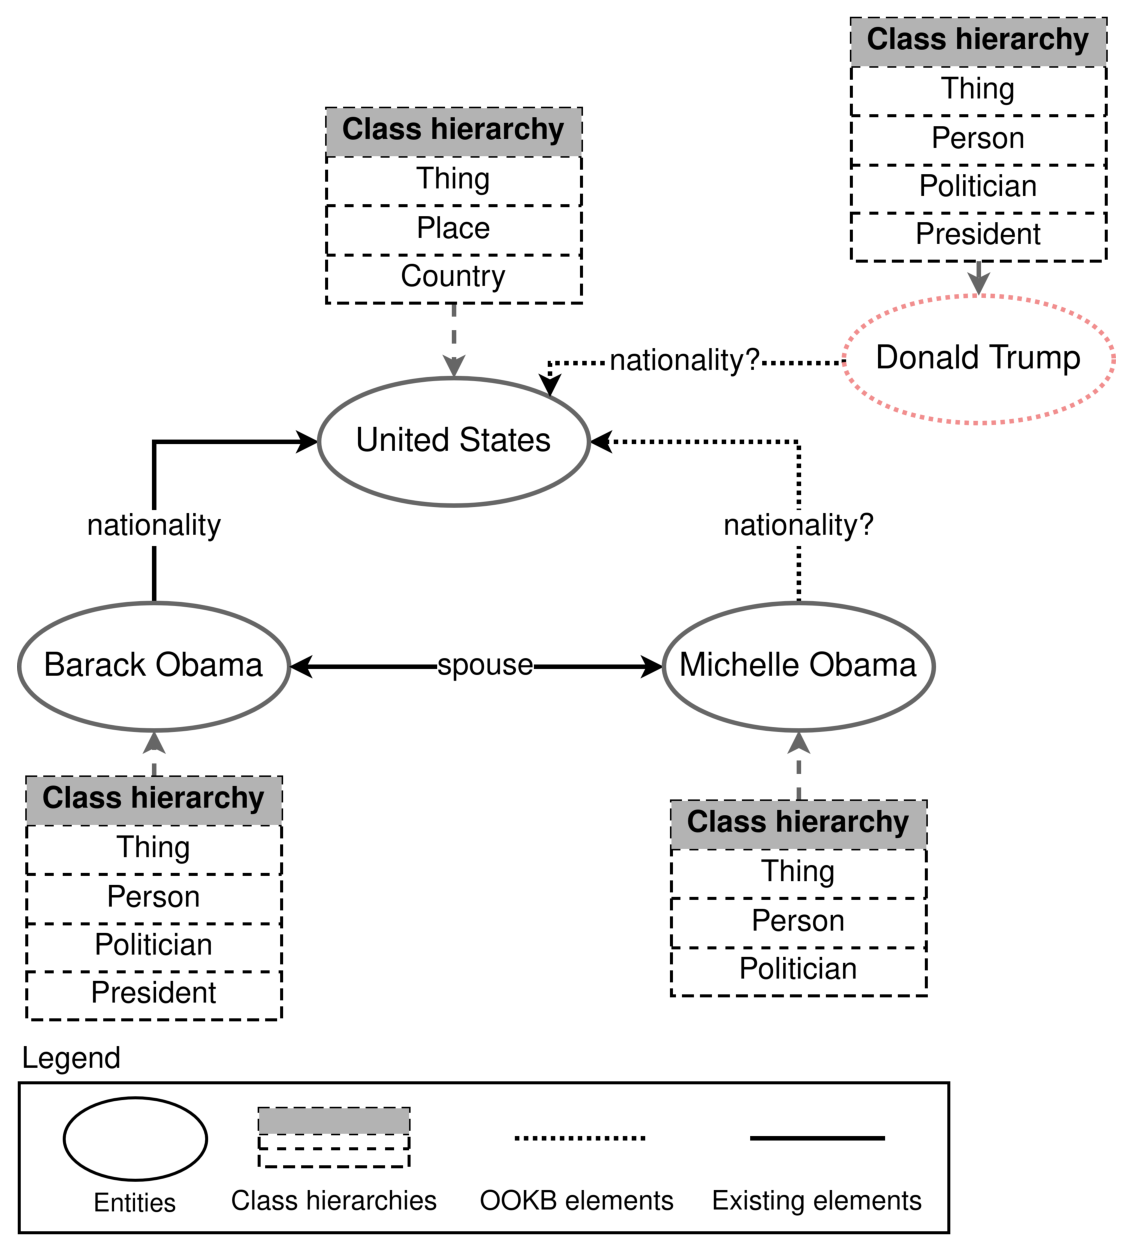
\includegraphics[width=.6\linewidth]{4_kbsintegrationdl/figures/KGCexample.eps}
    \caption{An example of KGC combining entity information and hierarchical information.}
    \label{fig:kgc_onto_example}
\end{figure}

Figure \ref{fig:kgc_onto_example} outlines the general idea of the proposal. Every entity contains its own ontological information. In this example, the class hierarchy of each entity is used as ontological information. While facts about a given entity $e$ are volatile and subject to change, its class hierarchy remains reasonably static throughout time. Moreover, class hierarchies are similar or even equal in those entities representing closely related concepts. \textit{Barack Obama} ($e_1$) and \textit{Donald Trump} ($e_2$) class hierarchies are equal, implying that they represent the same type of concept. For the entity \textit{Michelle Obama}, its class hierarchy is a subset of the class hierarchy of the aforementioned entities. Therefore, even though this entity does not represent a \textit{President}, it still holds a high resemblance with both $e_1$ and $e_2$. Considering the equality of the class hierarchies of entities $e_1$ and $e_2$, even though $e_2$ was not featured in the training set, analogical inference can be performed. The combination of the ontological background of the entity with its specific information makes it possible to leverage information about similar entities, leading the model to infer restrictions capable of enabling reasoning over OOKB entities. In the example depicted in Figure \ref{fig:kgc_onto_example}, even though the only known information about the entity \textit{Donald Trump} is its class hierarchy, it can be assessed whether the potential fact \textit{(DonaldTrump, nationality, UnitedStates)} holds based on its resemblance with the known fact \textit{(BarackObama, nationality, UnitedStates)}. 

%%%INICIO BLOQUE PAPER

\subsection{Semantic-Based Initialization for Out-Of-Knowledge-Base Entity Reasoning}

\label{4_sec:semantic_initialization}
\begin{figure}
    \centering
    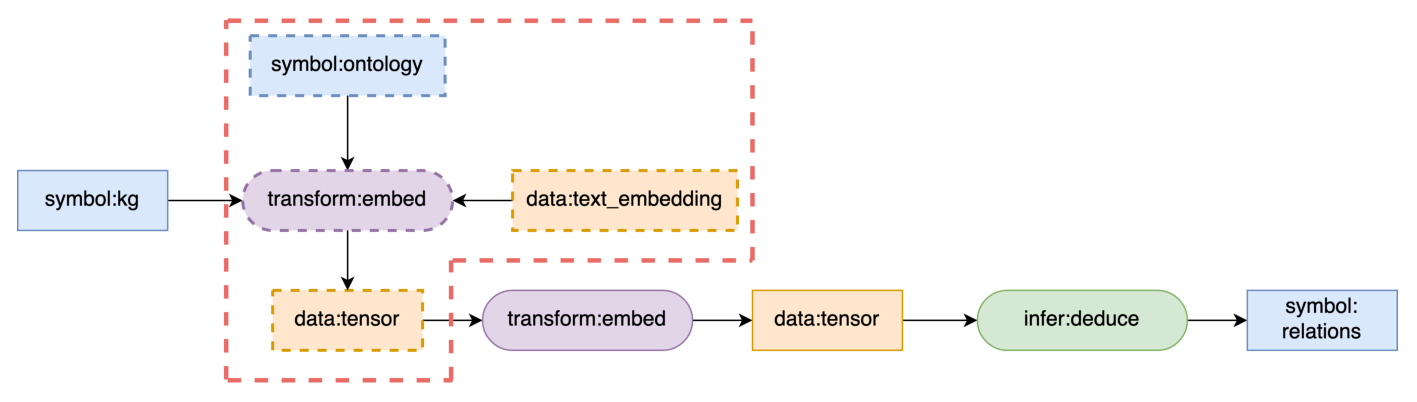
\includegraphics[width=\linewidth]{4_kbsintegrationdl/figures/VanBekkum_KGEOnto.eps}
    \caption{Boxology representation of the proposed hybrid KGE model. Dashed lines are used to highlight the added elements with respect to the baseline (Figure \ref{fig:van_bekkum_kgc_kge}).}
    \label{fig:box_krintodl}
\end{figure} 

Even though the introduction of ontological information solves the issue of OOKB entity reasoning, specific information about the unseen entities is also required to properly typify them. Moreover, unseen entities need to be represented in the same format as known entities to be processed by the KGE model. Figure \ref{fig:box_krintodl} shows the boxology representation of the proposed approach. Instead of directly feeding a set of facts in relational format to the KGE model like in the baseline model, an additional transformation layer is added to perform initialization (depicted as a red box). The proposed initialization method encodes not only ontological information, but specific semantic knowledge about each of the entities. From a formal representation standpoint, the proposed hybrid model may be perceived as more complex due to its increased number of boxes. However, it is worth noticing that the initialization is performed offline, thus not adding any complexity to the KGE model itself. Figure \ref{fig:semantic_based_initialization} depicts the three phases of the initialization: \textit{ontology retrieval}, \textit{entity knowledge encoding} and \textit{embedding composition}.

\begin{figure}
    \centering
    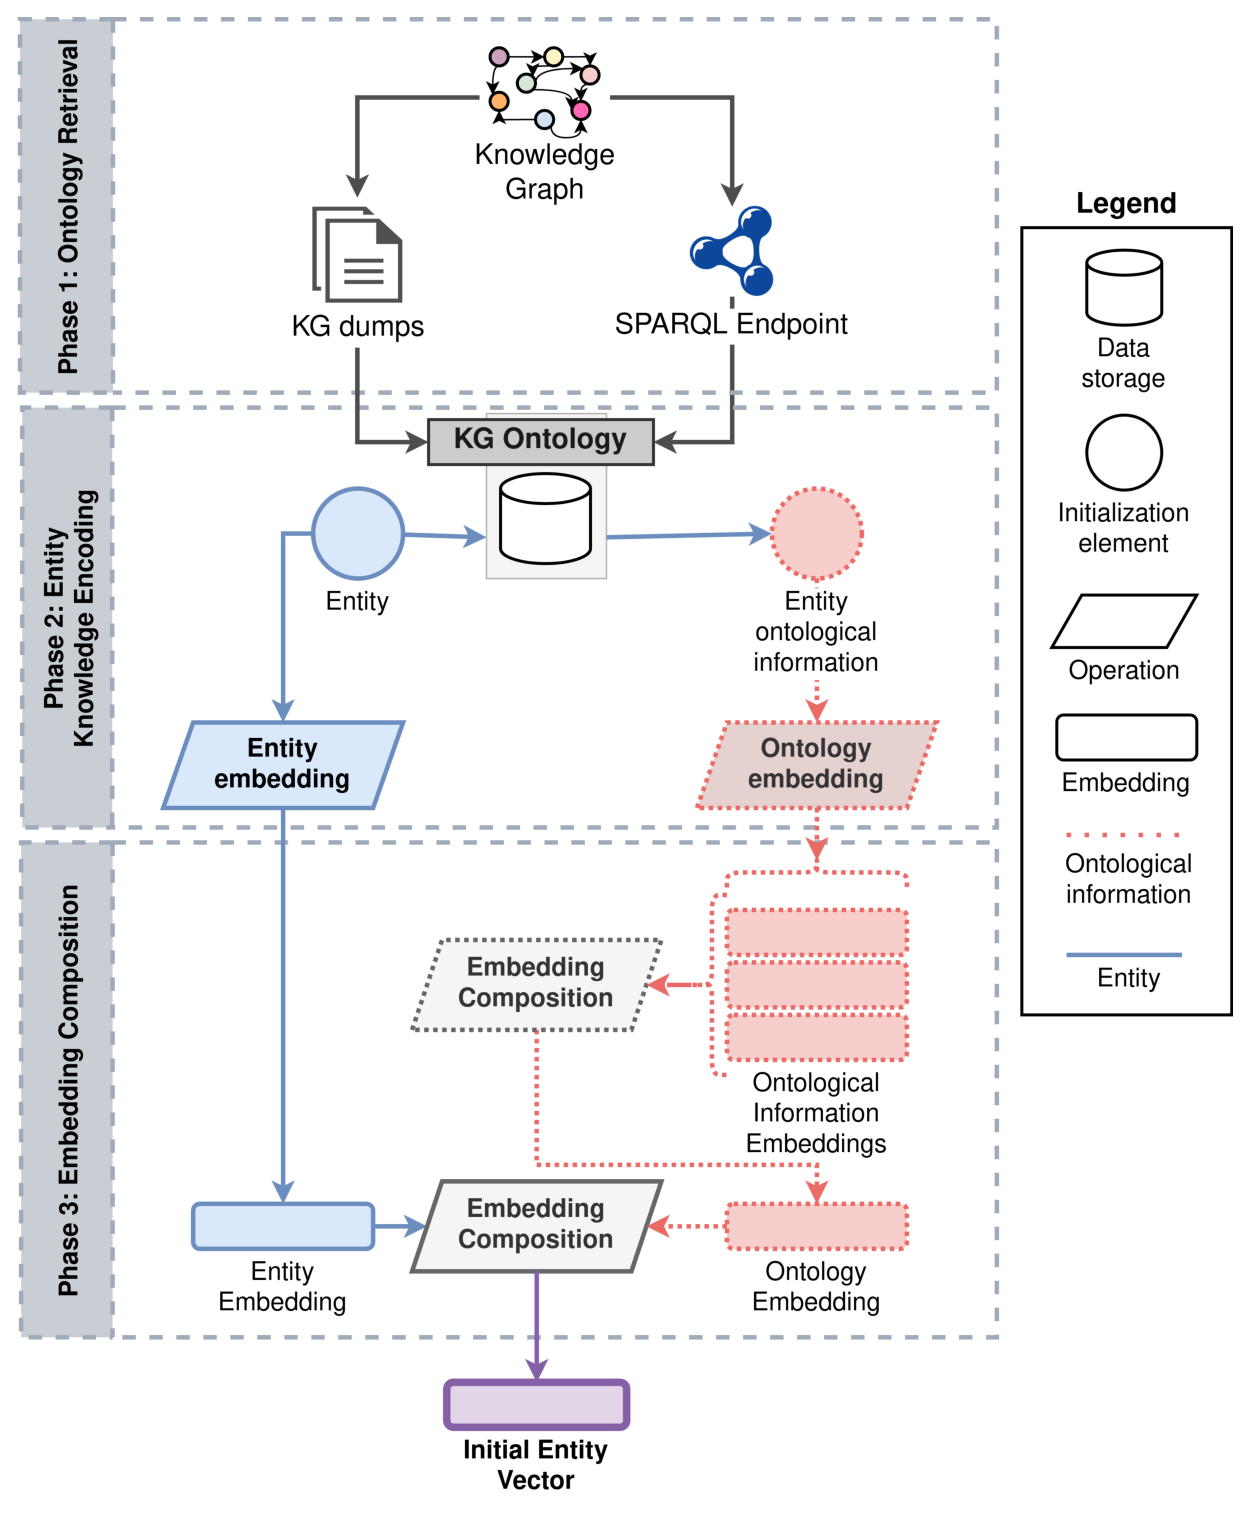
\includegraphics[width=.9\linewidth]{4_kbsintegrationdl/figures/Initialization_phases.eps}
    \caption{Overview of the three entity initialization phases.}
    \label{fig:semantic_based_initialization}
\end{figure}

\subsubsection{Theoretical Background.} \label{subsec:s4_theoretical_back}
As previously described, the purpose of KGE models is to subsymbollically represent the knowledge encoded in the KG, associating each entity and relation with a unique representation. One of the key features of the generated embeddings is that elements representing similar concepts must lead to similar encodings. From a technical standpoint, this constraint implies that if a pair of elements are conceptually similar, their corresponding embeddings should be close in the embedding distance. KGE models use specific scoring functions to ensure this restriction is met. While scoring functions vary amongst KGE models, two main categories can be defined: translational and bilinear. 

\begin{figure}[t!]
    \centering
    \subfigure[Translational model \label{fig:translational}]{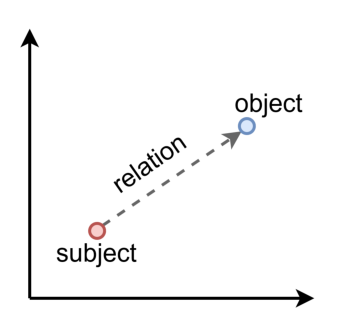
\includegraphics[height=1.5in]{4_kbsintegrationdl/figures/translational.eps}}
    \qquad
    \subfigure[Bilinear model \label{fig:bilinear}]{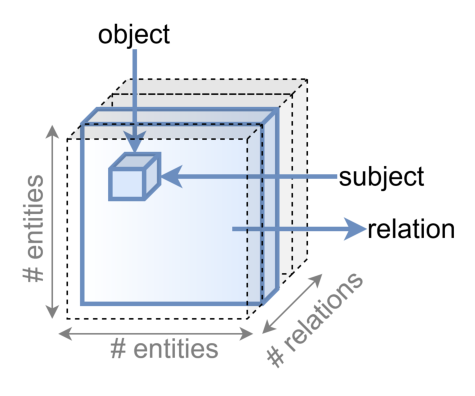
\includegraphics[height=1.5in]{4_kbsintegrationdl/figures/bilinear.eps}}
    \caption{Overview of the two main types of KGE models.}
    \label{fig:kge_overview}
\end{figure}

Translational models employ distance-based scoring functions. Figure \ref{fig:translational} depicts the core idea of translational models, where the relation between the subject and object entities is perceived as a translation operation. Entities and relations are modeled as vectors in ${\mathbb{R}}^{k}$, where $k$ is the dimension of the embeddings. As relation vectors $p$ are perceived as translation operations, a given fact $(s,p,o)$ holds when the distance between the embeddings $s+p$ and $o$ is minimal. The scoring function in Equation \ref{eq:trans_score} is formulated under the aforementioned constraint, which ensures that higher scores are assigned to lower distances:
\begin{equation}\label{eq:trans_score}
    f_p(s,o)=\|s + p - o\|_n
    \quad
    ( n \in \{1,2\})\,.
\end{equation} 

Bilinear models compute the plausibility of a given fact from the latent semantics and correlations existing between entities and relations. Figure \ref{fig:bilinear} showcases the foundation of bilinear models, where the KG is depicted as a tensor of dimensions $N_{entities} \times N_{entities} \times N_{relations}$. Each slice of the tensor models the pairwise interaction between the existing entities for a given relation $r$. Opposite to translational models, relations are depicted as matrices in $\mathbb{R}^{k_x k}$, where $k$ is the dimension of the embeddings. Entities follow the same representation criteria as translational models. Equation \ref{eq:bilinear_score} defines the scoring function employed by these models, where $M_p$ is the relation matrix , and $s$ and $o$ are the subject and object vector embeddings, respectively.

\begin{equation}\label{eq:bilinear_score}
    f_r(s,o)=s^T M_p o \,.
\end{equation}


%%%LOS RELATED WORKSSS
% The incremental six-step initialization procedure is depicted in Figure \ref{fig:overview}. These steps can be grouped into three different phases: \textbf{entity information retrieval, embedding generation} and \textbf{performance evaluation}


% Figure \ref{fig:overview} showcases the proposed incremental six-step procedure conducted to initialize and reason over OOKB entities. 
% \elvitodo{A lo mejor esa figura se podría modernizar, que está fea} These steps can be categorized into three phases: entity information retrieval, embedding generation and performance evaluation.

\subsubsection{Ontology Retrieval.} \label{subsec:s4_onto_retrieval}
Opposite to the volatility of KGs, ontologies provide stable, general information. Their role in the generation of KGs is crucial, but their application scope is usually limited to the introduction and creation of new elements of the graph. The information encoded in ontologies can be particularly beneficial for KGC, as they provide explicit restrictions about the type of entities featured in each relation, as well as additional information that can boost the inference process.

Ontologies comprise the following parts: individuals, classes, properties, relations, function terms, restrictions, rules, axioms, and events. Only individuals (or entities in the context of KGs), relations, and properties are considered by KGE models for the generation of representations. Therefore, a substantial number of components that could improve the final quality of the embeddings is dismissed.

Class hierarchies are at the core of both ontologies and KGs. During the introduction, entities are grouped into the class that better represents them conceptually. Classes are not atomic, but form a tree-like hierarchical structure, ranging from the most specific (or \textit{leaf}) classes to the \textit{root} class, which is shared by all entities in the graph. This taxonomical structure enables fine-grained distinctions between conceptually similar classes, as in Figure \ref{fig:kgc_onto_example}, where the entities \textit{Barack Obama} and \textit{Michelle Obama} are both \textit{Politicials}, but the first one is also a \textit{President}. Therefore, it provides a trade-off between the generality of the tree-like structure with the specificity of the different subclasses. 

While classes provide a general and unified framework, properties provide distinct, unique information about entities. KG facts are usually extracted from the interaction between two individuals by means of a property. Properties that relate an individual with a non-individual (i.e: a numerical value, a description, etc.) are usually discarded, even though this information could further enrich the final embeddings. Rules and axioms can also be encoded within the KGE model. In this case, axioms can be used to guide the training of the KGE model, ensuring the consistency of the predictions. Additionally, rules can also be used for training data augmentation, as new facts may be inferred from the existing KG. The newly inferred facts can then also be included as part of the training set.

Restrictions are also closely related with KGEs, as relation representations encode implicit constraints about the expected types of subject and object entities. However, the restrictions inferred by KGE models have a local scope, as they are based only on the facts contained in the training set. Therefore, these constraints may not be applicable to every fact that features the relation. Explicit restrictions about the relations can also be encoded jointly with their representations to deal with this shortcoming, improving the performance of the model on KGC.

Phase 1 of Figure \ref{fig:semantic_based_initialization} illustrates two different available paths for ontology retrieval: KG dumps or SPARQL queries. Currently, most of the publicly available KGs provide their data dumps, which includes not only the KG facts, but its ontology file along with extra documentation. Every entity and relation encoded in the KG is explicitly related to its corresponding ontological information, which reduces the retrieval time. Data dumps usually come compressed in a single file that can scale up to several terabytes, which can be undesirable in terms of computational resources. KGs usually provide a SPARQL endpoint, which enables information retrieval via queries. This approach is more efficient, as fewer resources are required and the target information can be retrieved directly with a single query. Nonetheless, using SPARQL queries may be discouraged in cases where the KG has a large size or if the number of SPARQL queries is elevated. 

\subsubsection{Entity Knowledge Encoding.}\label{subsec:s4_entity_encode}
The first phase of the proposed initialization focuses on obtaining the ontological information required to categorize each entity. While the existing OOKB entity reasoning approaches presented in Section \ref{4_sec:ontointro_kgc} are capable of generating highly representative embeddings, these representations lack any semantic information about the entity itself. Semantic information is highly relevant in this context, as it enriches the entity embeddings with an additional level of knowledge that can not be inferred otherwise. Despite this fact, most KGE models still rely on random initialization. 

One-hot vectors are an easy and straightforward replacement for random initialization. In this encoding, each entity is embedded as a vector of dimension $N$, where $N$ is the total number of entities. For every entity, a single vector can be created composed entirely of zeros except for a single one value in a given position, which is unique to each entity. While this encoding may be suitable for small KGs, it cannot be applied to large inputs, as the dimension of the embedding grows linearly with the size of the KG. Moreover, zero-valued initializations can hinder the convergence of the model to its optimal solution, and they do not encode semantic information about the entity.

Language models are a potential initialization alternative. These methods are capable of generating expressive, unique representations for words. Different paradigms can be identified amongst language models for the representation of words. Word2Vec \citep{word2vec} generates a single representation per token in the vocabulary, which hinders the representation of unseen words. FastText \citep{fasttext1,fasttext2} considers each word as a set of subparts called n-grams, assigning a representation for each of them. The final representation of a word is composed by the average of this n-grams. While FastText is capable of representing words that were not in the training corpus and still enable analogical reasoning, it still lacks the capability of correctly model polysemy. Language models, such as ElmO \citep{elmo} or BERT \citep{bert} solve all of the aforementioned issues, but the dimension of the resulting embeddings increases noticeably. Word2Vec embeddings tend to have a length of about 300, which scales up to 2048 on BERT. This dimension conflicts with the regular dimension of KGE vectors, which rarely exceed 200. Dimensionality reduction based on principal component analysis is a potential solution to the mismatch between the dimensions of KGE and word embedding outputs. However, it must be noted that reducing the dimension of a word embedding directly can affect its final expressivity. 

Another important dissimilarity between word and KG embeddings is that whereas word embeddings follow a token-based approach, KGE models are oblivious to the number of tokens that name an entity. Therefore, a composition method is needed that guarantees that all tokens that compose an entity are represented on its initial embedding. A potential solution for this issue would be to concatenate single representations of each entity token to generate the initial entity embedding. However, this solution is not feasible in the context of KGEs, as all entity embeddings must be equally dimensional. Averaging token representations to generate the initial entity embeddings provides a more fitting solution to this case.

The encoding process of this phase is outlined in Figure \ref{fig:semantic_based_initialization}. Alongside the initial entity embedding, feasible encodings for the ontology are also generated in this phase. The encoding of the ontological information depends on two factors: i) the type of ontological information selected, and ii) the targeted component of the KG (entity or relation). 

Class hierarchies only encompass entities, which are modelled as vectors by most KGE models. Therefore, a vector encoding must be also employed to represent class hierarchies. The simplest feasible solution uses one-hot vectors of dimension $O$, where $O$ is the number of classes that comprises the ontology. While simple, this representation is suitable for representing the class hierarchy of each entity, as it ensures the maintenance of the similarity between the embeddings of the classes of similar entities. Although valid, this codification presents two main shortcomings: i) it lacks semantic information about the concept represented by the class, and ii) its dimension grows linearly with the number of classes in the ontology. Word embeddings can also be used for class hierarchy embedding. In this scenario, each ontology class is encoded using its corresponding word embedding.

In the case of relations, matrices can be used for restriction encoding. Each relation can be codified as a matrix of dimensions $C \times C$, where $C$ is the total of leaf classes and restrictions that can be encoded using binary vectors. If the head class $i$ is restricted to the tail class $j$ through a relation, the cell $(i,j)$ should have a positive value denoting this restriction, and zero otherwise.



\subsubsection{Embedding Composition.} \label{subsec:s4_embedding_compo}
In this stage, semantic and ontological information are combined to generate the initial value of the entity, as shown in Figure \ref{fig:semantic_based_initialization}. First, the embeddings of the ontological information about the entity are flattened into a single representation. In the context of class hierarchies, an entity can belong to several different classes, each with a unique representation. Hence, the embeddings of the entity classes must be combined into a single embedding. Different vector composition techniques can be used for this task. Averaging all class embeddings is one potential solution, although this approach does not encode the hierarchical information of the ontology classes. Weighted average can be used instead, potentially introducing the hierarchical properties of the ontology in the final representation.

As stated in the previous phase, the encoding method must be aligned with the target component of the KG. If the ontological information is embedded alongside the KGE, then the encoding method must be compliant with the dimension restrictions of the model. While in this initialization the focus is on entity embeddings, the same restriction applies for relations. Three composition procedures can be employed to combine the ontological information alongside the embeddings of the KGE model:
\begin{itemize}
    \item \textit{Concatenation:} The simplest approach is to append the representations of each class to generate a high-dimensional embedding. This procedure ensures that a section of the embedding remains static throughout the training, and that its equal across entities that share ontological information. This ensures a similarity in the final representations of similar entities. Therefore, if the dimension specified by the KGE model for the embeddings is $d_T$, the following constraint must be met:
    \begin{equation}
        d_O+d_M=d_T\,,
    \end{equation}
    where $d_M$ is the dimension of the entity embeddings and $d_O$ is the dimension of the ontological information embedding. In this scenario, $d_O$ and $d_M$ are not required to have the same dimension. While this approach is suitable for the problem, the training time of the model increases due to the growth in the embedding size. Additionally, the optimal dimensions for the ontological and entity representations must be determined beforehand to ensure a fair tradeoff between general and specific knowledge.
    
    \item \textit{Average:} In this approach, both representations are averaged into a single embedding. Therefore, both entity and ontological representations must have the same dimension, following the constraint:
    \begin{equation}
        d_T = d_O = d_M.
    \end{equation}
    The simplest way to ensure this condition is met is to use the same embedding model for both entity and ontology embeddings. Otherwise, either reduction or zero-padding may be necessary to ensure that both representations have the same dimension before averaging them. This approach assigns equal importance to general and specific information. As all embedding dimensions are equal in this scenario, performing dimension reduction is less penalizing than in the previous case.
    
    \item \textit{Weighted Average:} While averaging solves the dimensionality problem existing in the concatenation option, this technique is still oblivious to the balance between general and specific information. Weighted average solves this issue, enabling the possibility of assigning different relevance values to specific and ontological information. While averaging and assigning the same weight to both representations may be perceived as the fairest approach, it may not be optimal for the performance of the KGE model. As in the previous case, both entity and ontological information embeddings must have the same dimension. In addition, the following composition constraint must be met:
    \begin{equation}
        T = \frac{\lambda \times O + (1 - \lambda) \times M}{2}\,,
    \end{equation}
    where $T$ is the final representation, $\lambda$ is the assigned weight, and $O$ and $M$ are the ontological information and entity embeddings, respectively. This method maintains the balancing benefits of concatenation while maintaining a stable dimension for the embeddings. Nonetheless, it rises a new challenge: computing the optimal value of $\lambda$. This value can be manually defined or treated as an additional training parameter to optimize.
\end{itemize}

The proposed initialization approach is model-agnostic, and can subsequently be encoded alongside any KGE model. However, from a conceptual standpoint, it may not be suitable for any proposal. In translational models, optimization is performed by reducing the distance between the result of a translation operation and a target value, following an entirely arithmetic approach. As neither latent semantics nor correlations are considered, the introduction of ontological information may be detrimental for the performance of the model.

Bilinear models base their predictions on the exploitation of latent semantics and implicit correlations between elements. Enriching the semantic information available to the model during training time can potentially be translated into an improvement on its performance. Moreover, the inclusion of ontological information can add an exploratory layer to KGE models in addition to their exploitative behavior.

\subsection{Evaluation}\label{4_sec:experiments}
%%AQUI EXPLICAMOS YA LOS MODELOS EXACTOS SOBRE LOS QUE SE EVALUA Y LOS DATASETES
\begin{table}[h]
\resizebox{\linewidth}{!}{
\begin{tabular}{|c|c|c|c|c|}
\hline
\textbf{Model name} & \textbf{Model type}        & \begin{tabular}[c]{@{}c@{}}\textbf{Embedding} \\ \textbf{Dimensions}\end{tabular} & \begin{tabular}[c]{@{}c@{}}\textbf{Scoring} \\ \textbf{Function}\end{tabular} & \begin{tabular}[c]{@{}c@{}}\textbf{Complexity} \\ \textbf{Order}\end{tabular}\\ \hline
TransE \citep{transe}    & Translational &\begin{tabular}[c]{@{}c@{}}$h,t \in \R ^d$ \\ $r \in \R ^d$\end{tabular}  &$- {\lVert h + r - t \rVert}_{\frac{1}{2}} $&$\mathcal{O}(d)$\\ \hline
DistMult \citep{distmult}   & Bilinear & \begin{tabular}[c]{@{}c@{}}$h,t \in \R ^d$ \\ $r \in \R ^d$\end{tabular}  & $h^Tdiag(r)t$&$\mathcal{O}(d)$\\ \hline
ComplEx \citep{complex}    & Bilinear &\begin{tabular}[c]{@{}c@{}}$h,t \in \C^d$ \\ $r \in \C^d$\end{tabular} & $Re(h^T diag(r) \compconj{t})$ &$\mathcal{O}(d)$\\ \hline
ANALOGY \citep{analogy}    & Bilinear &\begin{tabular}[c]{@{}c@{}}$h,t \in \R ^d$ \\ $r \in \R ^d$\end{tabular} &$h^T M_r t$&$\mathcal{O}(d)$\\\hline
SimplE \citep{simple}    & Bilinear & \begin{tabular}[c]{@{}c@{}}$h,t \in \R^d$ \\ $r,r^{-1} \in \R^d$\end{tabular}& $\frac{1}{2}[(h r t^T) + (h r^{-1} t)] $&$\mathcal{O}(d)$\\ \hline
\end{tabular}

\caption{Summary of the models considered for evaluation. Head and tail entity embeddings are shown as \textit{h} and \textit{t}, respectively. Relations whose embedding is vectorial are represented by an \textit{r}, while relation matrices are defined as $M_r$. The embedding dimension is denoted by \textit{d}. \label{tab:kge_experiment_model_summary}} 
}
\end{table}

The proposed initialization model is evaluated on five different KGE models. Considering the semantic nature of the proposed method, the experimentation primarily focuses on bilinear models. Table \ref{tab:kge_experiment_model_summary} summarizes the properties of each model. Section \ref{4_sec:ontointro_kgc} provided some references of approaches capable of performing OOKB entity reasoning. However, these approaches are not directly comparable with the method proposed due to a fundamental conceptualization difference. The proposals presented in Section \ref{4_sec:ontointro_kgc} are KGE models themselves, specifically designed for OOKB entity reasoning. On the contrary, the proposed method is not a KGE model by itself, and can be implemented across a wide variety of KGE models. In semantic-based initialization, OOKB entity reasoning is an induced benefit, but the final goal is to encode explicit background knowledge to overcome the existing limitations within KGE models.

Semantic-based initialization is evaluated on two triple classification datasets: FB13 \citep{neuraltensornetwork,Bollacker:2008:FCC:1376616.1376746} and WN11 \citep{Miller95wordnet:a}. These datasets contain facts from 13 and 11 relations extracted from Freebase and WordNet KGs, respectively. For each model reported in Table \ref{tab:kge_experiment_model_summary}, the optimal parameters reported by their authors are used. Similarly, the optimization algorithms recommended by the original authors are used: Adam \cite{adam} for FB13, and ADAGRAD \cite{adagrad} for WN11.

Triple classification is used to evaluate  the semantic-based initialization. Three different metrics are reported to assess the performance of the different KGE models in combination with the proposed initialization:

\begin{itemize}
    \item \textit{Recall} determines the proportion of true facts that are actually evaluated as true by the KGE model. Being \textit{TP} and \textit{FN} the number of true facts correctly and incorrectly classified respectively, recall can be computed as:
    \begin{equation}
        Recall = \frac{TP}{TP+FN}
    \end{equation}
    
    \item \textit{Average Precision (AP)} weights precision and recall increment of the model across different threshold values $t$. It provides an overall measurement of the model's classification while penalizing biased predictions. It is calculated as follows:
    \begin{equation}
        AP = \sum_{t} (R_t - R_{t-1}) \times P_t \,,
    \end{equation}
    where $R$ denotes the recall value, and $P$ represents the precision, computed as:
    \begin{equation}
        Precision = \frac{TP}{TP+FP} \,,
    \end{equation}
    \textit{FP} depicts the number of unfeasible facts predicted as true by the KGE model.
    
    \item \textit{F1 Score} is the harmonic mean between precision and recall, and serves as an indicator of the model's accuracy. It can be computed as:
    \begin{equation}
        F1 \; Score = \frac{2 (P \times R)}{(P + R)}
    \end{equation}
\end{itemize}

Semantic-based initialization is evaluated following an incremental approach. First, simple entity initialization is performed, replacing random initialization with word embedding based initialization. Simple entity initialization is then extended to include ontological information, which is embedded alongside the entities. Finally, semantic-based initialization is evaluated for OOKB entity reasoning.

\subsubsection{Simple Entity Initialization.}

\begin{table} 
\centering
\resizebox{.8\linewidth}{!}{
\begin{tabular}{l|c|c|c|c|c|c|}
\cline{2-7}
                                                                & \multicolumn{3}{c|}{FB13} & \multicolumn{3}{c|}{WN11} \\ \cline{2-7} 
                                                                & TCAP  & Recall & F1 Score & TCAP  & Recall & F1 Score \\ \hline
\multicolumn{1}{|l|}{\textit{ComplEx}}                          & 0.78  & 0.65   & 0.68     & 0.71  & 0.58   & 0.62     \\
\multicolumn{1}{|l|}{\textit{CompEx + SEI}}   & 0.76  & 0.64   & 0.67     & 0.76  & 0.6    & 0.64     \\ \hline
\multicolumn{1}{|l|}{\textit{DistMult}}                         & 0.71  & 0.61   & 0.64     & 0.68  & 0.58   & 0.61     \\
\multicolumn{1}{|l|}{\textit{DistMult + SEI}} & 0.71  & 0.61   & 0.64     & 0.68  & 0.58   & 0.61     \\ \hline
\multicolumn{1}{|l|}{\textit{TransE}}                           & 0.72  & 0.58   & 0.62     & 0.82  & 0.65   & 0.69     \\
\multicolumn{1}{|l|}{\textit{TransE + SEI}}   & 0.72  & 0.58   & 0.62     & 0.83  & 0.65   & 0.69     \\ \hline
\multicolumn{1}{|l|}{\textit{ANALOGY}}                          & 0.65  & 0.52   & 0.58     & 0.67  & 0.58   & 0.59     \\
\multicolumn{1}{|l|}{\textit{ANALOGY + SEI}}  & 0.68  & 0.58   & 0.61     & 0.68  & 0.56   & 0.6      \\ \hline
\multicolumn{1}{|l|}{\textit{SimplE}}                           & 0.77  & 0.65   & 0.67     & 0.48  & 0.49   & 0.49     \\
\multicolumn{1}{|l|}{\textit{SimplE + SEI}}   & 0.74  & 0.64   & 0.67     & 0.6   & 0.53   & 0.55     \\ \hline
\end{tabular}}
\caption{Triple classification average precision. recall. and F1 score with and without entity initialization (marked as +SEI)}
\label{tab:exp_entity_init}
\end{table}

A pretrained Word2Vec model is used to obtain the initial embeddings for the entity set $\mathcal{E}$. By using a pretrained model, the computational cost of the proposal remains low. As stated in Section \ref{subsec:s4_entity_encode}, entities can be compound, while the selected Word2Vec model is tokenized. Therefore, given an entity $e \in \mathcal{E}$, its initial embedding is obtained by averaging all the tokens contained in $e$. First, the entity vocabulary $V$ is created, containing all unique entity tokens. For each token $t \in V$, its representation is extracted from the pretrained Word2Vec model, and stored in a dictionary of tuples of the form $(token, embedding)$.

The selected Word2Vec model provides 300-dimension representations. The KGE models selected for evaluation use embedding dimensions that range from 100 to 200. Dimension reduction based on principal component analysis is performed to fit the dimension of the token embeddings to 200. Then, for each entity $e \in \mathcal{E}$, its tokens $t \in e$ are extracted from the previously constructed dictionary and averaged afterwards to generate a single representation. Those entities where none of its tokens is contained in the Word2Vec model's vocabulary are initialized using a randomized normal distribution.

Table \ref{tab:exp_entity_init} reports the TCAP, F1 score and recall for each model with and without simple entity initialization (marked as + SEI).

\subsubsection{Semantic-Based Initialization.}
The class hierarchy of entities is selected as ontological information in the second experimentation stage, as it can be easily integrated within the previously initialized entity embeddings. SPARQL endpoints are used to retrieve the class hierarchy of each entity. For the entities in WN11, its homonym ontology is applied, which splits the entities into four classes according to their word type: nouns, adjectives, verbs and adverbs. For FB13, two different ontologies are considered. Freebase is currently integrated within the Google Knowledge Graph, thus inheriting its ontology. The GKG API was employed to retrieve the classes of each FB13 entity, identifying a total of 64 classes. The root class \textit{Thing} is assigned to those entities where no leaf classes are specified.

An additional ontology is considered for FB13 to study the existing dependency between the complexity of the class hierarchy and the results achieved by the KGE model. DBpedia ontology is selected, having a total number of 685 different classes. The DBpedia SPARQL endpoint is used to retrieve the class hierarchy of each entity. As this ontology is external to FB13, each entity's class hierarchy cannot be directly obtained. The SPARQL query in Listing \ref{lst:sparql} is executed for each entity, exchanging the label value according to each entity $e \in \mathcal{E}$. The class hierarchy of each entity is saved in a dictionary of tuples of the form $(entity, [classes])$. From the total 685 classes of the DBpedia ontology, only 197 are featured in the class hierarchies of the entities in FB13. As in the previous case, the root class \textit{Thing} is assigned to those entities where no class information is available.

\begin{lstlisting}[captionpos=b, float=tp,floatplacement=tbp, caption=Example of a SPARQL query used to retrieve the class hierarchy of the entity ``Albert Einstein''., label=lst:sparql,basicstyle=\ttfamily,frame=single]
PREFIX dbr: <http://dbpedia.org/resource/>
SELECT DISTINCT ?class
WHERE {
 ?item rdfs:label "Albert Einstein"@en .
 ?item rdf:type ?class.
 ?class a owl:Class.
}
\end{lstlisting}

After retrieving the class hierarchy of the entities, the same pretrained Word2Vec model employed for simple entity initialization is used for encoding the ontology classes. Similarly to the previous case, for those classes composed by more than one word, average composition is applied to generate a single representation per class. The embeddings of each class are stored in a dictionary of tuples of the form $(class, embedding)$. Dimension reduction is also performed on the class embeddings to ensure equality between the dimensions of the entity and ontological embeddings.

For each $e \in \mathcal{E}$, its list of classes $C$ is obtained. Then, for each $c \in C$, its corresponding embedding is retrieved is embedding from the corresponding dictionary, then averaged to produce a single representation. A matrix of dimensions $N_e \times d_T$ is obtained as a result, being $N_e$ the number of entities and $d_T$ the dimension of the KGE model embeddings. Each entity embedding is then averaged with its corresponding ontology embedding on each training iteration, generating a single representation per entity during training time. Whereas the entity embeddings are model parameters and are subsequently updated during training, ontology embeddings remain static. This constraint ensures that the ontological information of the entities remains constant and that the equality between the class hierarchies of similar entities is always met.

\begin{table} 
\centering
\resizebox{.85\linewidth}{!}{
\begin{tabular}{l|c|c|c|c|c|c|}
\cline{2-7}
\textit{}                                                                & \multicolumn{3}{c|}{FB13} & \multicolumn{3}{c|}{WN11} \\ \cline{2-7} 
\textit{}                                                                & TCAP  & Recall & F1 Score & TCAP  & Recall & F1 Score \\ \hline
\multicolumn{1}{|l|}{\textit{ComplEx + DBOnt}}                           & 0.65  & 0.6    & 0.62     & -     & -      & -        \\
\multicolumn{1}{|l|}{\textit{ComplEx + GKGOnt}}                          & 0.74  & 0.62   & 0.65     & -     & -      & -        \\
\multicolumn{1}{|l|}{\textit{ComplEx + WNOnt}}                           & -     & -      & -        & 0.75  & 0.58   & 0.64     \\
\multicolumn{1}{|l|}{\textit{CompEx + DBOnt + SEI}}    & 0.73  & 0.62   & 0.65     & -     & -      & -        \\
\multicolumn{1}{|l|}{\textit{ComplEx + GKGOnt + SEI}}  & 0.73  & 0.61   & 0.63     & -     & -      & -        \\
\multicolumn{1}{|l|}{\textit{ComplEx + WNOnt + SEI}}   & -     & -      & -        & 0.76  & 0.6    & 0.65     \\ \hline
\multicolumn{1}{|l|}{\textit{DistMult + DBOnt}}                          & 0.71  & 0.62   & 0.64     & -     & -      & -        \\
\multicolumn{1}{|l|}{\textit{DistMult + GKGOnt}}                         & 0.74  & 0.62   & 0.65     & -     & -      & -        \\
\multicolumn{1}{|l|}{\textit{DistMult + WNOnt}}                          & -     & -      & -        & 0.65  & 0.57   & 0.6      \\
\multicolumn{1}{|l|}{\textit{DistMult + DBOnt + SEI}}  & 0.71  & 0.62   & 0.64     & -     & -      & -        \\
\multicolumn{1}{|l|}{\textit{DistMult + GKGOnt + SEI}} & 0.75  & 0.61   & 0.62     & -     & -      & -        \\
\multicolumn{1}{|l|}{\textit{DistMult + WNOnt + SEI}}  & -     & -      & -        & 0.75  & 0.6    & 0.64     \\ \hline
\multicolumn{1}{|l|}{\textit{ANALOGY + DBOnt}}                           & 0.67  & 0.6    & 0.62     & -     & -      & -        \\
\multicolumn{1}{|l|}{\textit{ANALOGY + GKGOnt}}                          & 0.68  & 0.6    & 0.63     & -     & -      & -        \\
\multicolumn{1}{|l|}{\textit{ANALOGY + WNOnt}}                           & -     & -      & -        & 0.7   & 0.58   & 0.6      \\
\multicolumn{1}{|l|}{\textit{ANALOGY + DBOnt + SEI}}   & 0.67  & 0.6    & 0.62     & -     & -      & -        \\
\multicolumn{1}{|l|}{\textit{ANALOGY + GKGOnt + SEI}}  & 0.68  & 0.6    & 0.62     & -     & -      & -        \\
\multicolumn{1}{|l|}{\textit{ANALOGY + WNOnt + SEI}}   & -     & -      & -        & 0.64  & 0.55   & 0.59     \\ \hline
\multicolumn{1}{|l|}{\textit{SimplE + DBOnt}}                            & 0.63  & 0.6    & 0.61     & -     & -      & -        \\
\multicolumn{1}{|l|}{\textit{SimplE + GKGOnt}}                           & 0.76  & 0.63   & 0.66     & -     & -      & -        \\
\multicolumn{1}{|l|}{\textit{SimplE + WNOnt}}                            & -     & -      & -        & 0.6   & 0.55   & 0.57     \\
\multicolumn{1}{|l|}{\textit{SimplE + DBOnt + SEI}}    & 0.66  & 0.6    & 0.62     & -     & -      & -        \\
\multicolumn{1}{|l|}{\textit{SimplE + GKGOnt + SEI}}   & 0.74  & 0.61   & 0.65     & -     & -      & -        \\
\multicolumn{1}{|l|}{\textit{SimplE + WNOnt + SEI}}    & -     & -      & -        & 0.62  & 0.54   & 0.58     \\ \hline
\end{tabular}
}
\caption{Triple classification average precision per instance model with and without entity initialization and ontology introduction. For Freebase, two different ontologies are used: DBOnt refers to the DBpedia Ontology, and GKGOnt to the Google Knowledge Graph Ontology.}
\label{tab:exp_ont_intro}
\end{table}

This second experimentation stage is evaluated only on the bilinear models. Table \ref{tab:exp_ont_intro} reports the metrics achieved by each model on each ontology.

\subsubsection{OOKB Entity Reasoning.}
The third and final experimentation stage evaluates the capacity of the proposed semantic-based initialization to reason over facts containing OOKB entities. 1500 entities are randomly sampled from the total entity set $\mathcal{E}$ of both FB13 and WN11 to generate the OOKB entity set. All facts containing exactly one OOKB are withdrawn from the training, validation, and test sets, generating a new set of facts composed by one known and one OOKB entity. This ensures that OOKB entities remain entirely anonymous to the model. Facts containing two OOKB entities are not considered.

\begin{table} 
\centering
\begin{tabular}{l|c|c|}
\cline{2-3}
\textit{}                                       & FB13    & WN11    \\ \hline
\multicolumn{1}{|l|}{\textit{training facts}}   & 300,134 & 103,789 \\ \hline
\multicolumn{1}{|l|}{\textit{validation facts}} & 11,366  & 4,803   \\ \hline
\multicolumn{1}{|l|}{\textit{test facts}}       & 45,793  & 19,364  \\ \hline
\multicolumn{1}{|l|}{\textit{OOKB facts}}      & 34,319  & 19,722  \\ \hline
\end{tabular}
\caption{Number of examples per set and dataset. All training facts are positive, whereas validation, test, and OOKB facts contain an equal proportion of positive and negative examples.}
\label{tab:OOKB_proportions}
\end{table}

As the training set contains only true facts, the resulting OOKB test set is severely imbalanced, with the number of positive examples outnumbering the negative ones. Therefore, to maintain the proportion of the fully known test set, which has the same number of positive and negative examples, a corrupted sample is generated from each fact retrieved from the training set. The known entity of each fact is randomly swapped with another entity from the known set to create negative (or unfeasabile) facts, following the local closed-world assumption \citep{Reiter1978}. Table \ref{tab:OOKB_proportions} summarizes the number of examples of each set on the two datasets.

In this evaluation, random initialization is not considered, as the introduction of facts containing OOKB entities requires entity initialization to exploit the semantics contained in word embeddings to extend this knowledge to unseen entities. Ontological information is also required, as the generalization capacity of the KGE model is directly linked to its introduction. Each model is evaluated over the fully known and the OOKB test set. Table \ref{tab:OOKB_exp} summarizes the results of the third experimentation stage.

\begin{table}

\centering
\resizebox{.8\linewidth}{!}{
 \begin{tabular}{l|c|c|c|c|c|c|}
\cline{2-7}
                                                 & \multicolumn{6}{c|}{FB13}                                      \\ \cline{2-7} 
                                                 & \multicolumn{3}{c|}{Known set} & \multicolumn{3}{c|}{OOKB set} \\ \cline{2-7} 
\textit{}                                        & TCAP   & Recall   & F1 Score   & TCAP   & Recall   & F1 Score  \\ \hline
\multicolumn{1}{|l|}{\textit{ComplEx + DBOnt}}   & 0.75   & 0.63     & 0.66       & 0.63   & 0.5      & 0.55      \\
\multicolumn{1}{|l|}{\textit{ComplEx + GKGOnt}}  & 0.72   & 0.61     & 0.65       & 0.75   & 0.58     & 0.65      \\ \hline
\multicolumn{1}{|l|}{\textit{DistMult + DBOnt}}  & 0.76   & 0.62     & 0.65       & 0.6    & 0.6      & 0.59      \\
\multicolumn{1}{|l|}{\textit{DistMult + GKGOnt}} & 0.62   & 0.6      & 0.6        & 0.71   & 0.5      & 0.53      \\ \hline
\multicolumn{1}{|l|}{\textit{ANALOGY  + DBOnt}}  & 0.74   & 0.63     & 0.65       & 0.6    & 0.48     & 0.62      \\
\multicolumn{1}{|l|}{\textit{ANALOGY + GKGOnt}}  & 0.73   & 0.62     & 0.66       & 0.74   & 0.55     & 0.53      \\ \hline
\multicolumn{1}{|l|}{\textit{SimplE + DBOnt}}    & 0.69   & 0.6      & 0.63       & 0.61   & 0.47     & 0.53      \\
\multicolumn{1}{|l|}{\textit{SimplE + GKGOnt}}   & 0.77   & 0.63     & 0.67       & 0.71   & 0.54     & 0.6   \\
\hline
\end{tabular}}

\caption{TCAP, Recall, and F1 Score for the Freebase dataset.} \label{tab:ookb_fb}

\bigskip

\resizebox{.8\linewidth}{!}{
\begin{tabular}{l|c|c|c|c|c|c|}
\cline{2-7}
                                                                        & \multicolumn{6}{c|}{WN11}                                      \\ \cline{2-7} 
                                                                        & \multicolumn{3}{c|}{Known set} & \multicolumn{3}{c|}{OOKB set} \\ \cline{2-7} 
\textit{}                                                               & TCAP   & Recall   & F1 Score   & TCAP   & Recall   & F1 Score  \\ \hline
\multicolumn{1}{|l|}{\textit{ComplEx + WNOnt}}  & 0,75   & 0,61     & 0,64       & 0,51   & 0,5      & 0,64      \\ \hline
\multicolumn{1}{|l|}{\textit{DistMult + WNOnt}} & 0,72   & 0,59     & 0,63       & 0,54   & 0,5      & 0,65      \\ \hline
\multicolumn{1}{|l|}{\textit{ANALOGY + WNOnt}}  & 0,65   & 0,58     & 0,59       & 0,52   & 0,51     & 0,51      \\ \hline
\multicolumn{1}{|l|}{\textit{SimplE + WNOnt}}   & 0,62   & 0,55     & 0,57       & 0,52   & 0,51     & 0,52      \\ \hline
\end{tabular}
}
\caption{TCAP, Recall, and F1 Score for the WordNet dataset.} \label{tab:ookb_wn}

\caption{Top: (a) metrics obtained for the Freebase dataset. DBOnt refers to the DBpedia ontology, and GKGOnt to the Google Knowledge Graph Ontology. Bottom: (b) metrics obtained for the WordNet dataset. Entity initialization is used in all instances}
\label{tab:OOKB_exp}
\end{table}

\subsection{Result Analysis}\label{4_sec:results}
%%AÑADIR PERFORMANCE ASSESSMENT AQUI
\subsubsection{Simple Entity Initialization.}
As reported in Table \ref{tab:exp_entity_init}, simple entity initialization induces a slight improvement in most of the studied models. Initialization using semantically enriched representations, alongside with the information provided by the training facts, leads to more expressive representations. This improvement on the final expressivity of the embeddings is reflected in the results, as evidenced by the TCAP increment in ComplEx and SimplE in WN11. In the case of SimplE, the improvement is particularly remarkable, as TCAP increases from 48\% up to 62\%. In ComplEx, the improvement is close to 4.5\%, which is less noticeable but still significant. In FB13, the results remain fairly similar with and without initialization across the reported metrics.

\begin{figure}[t]
    \centering
    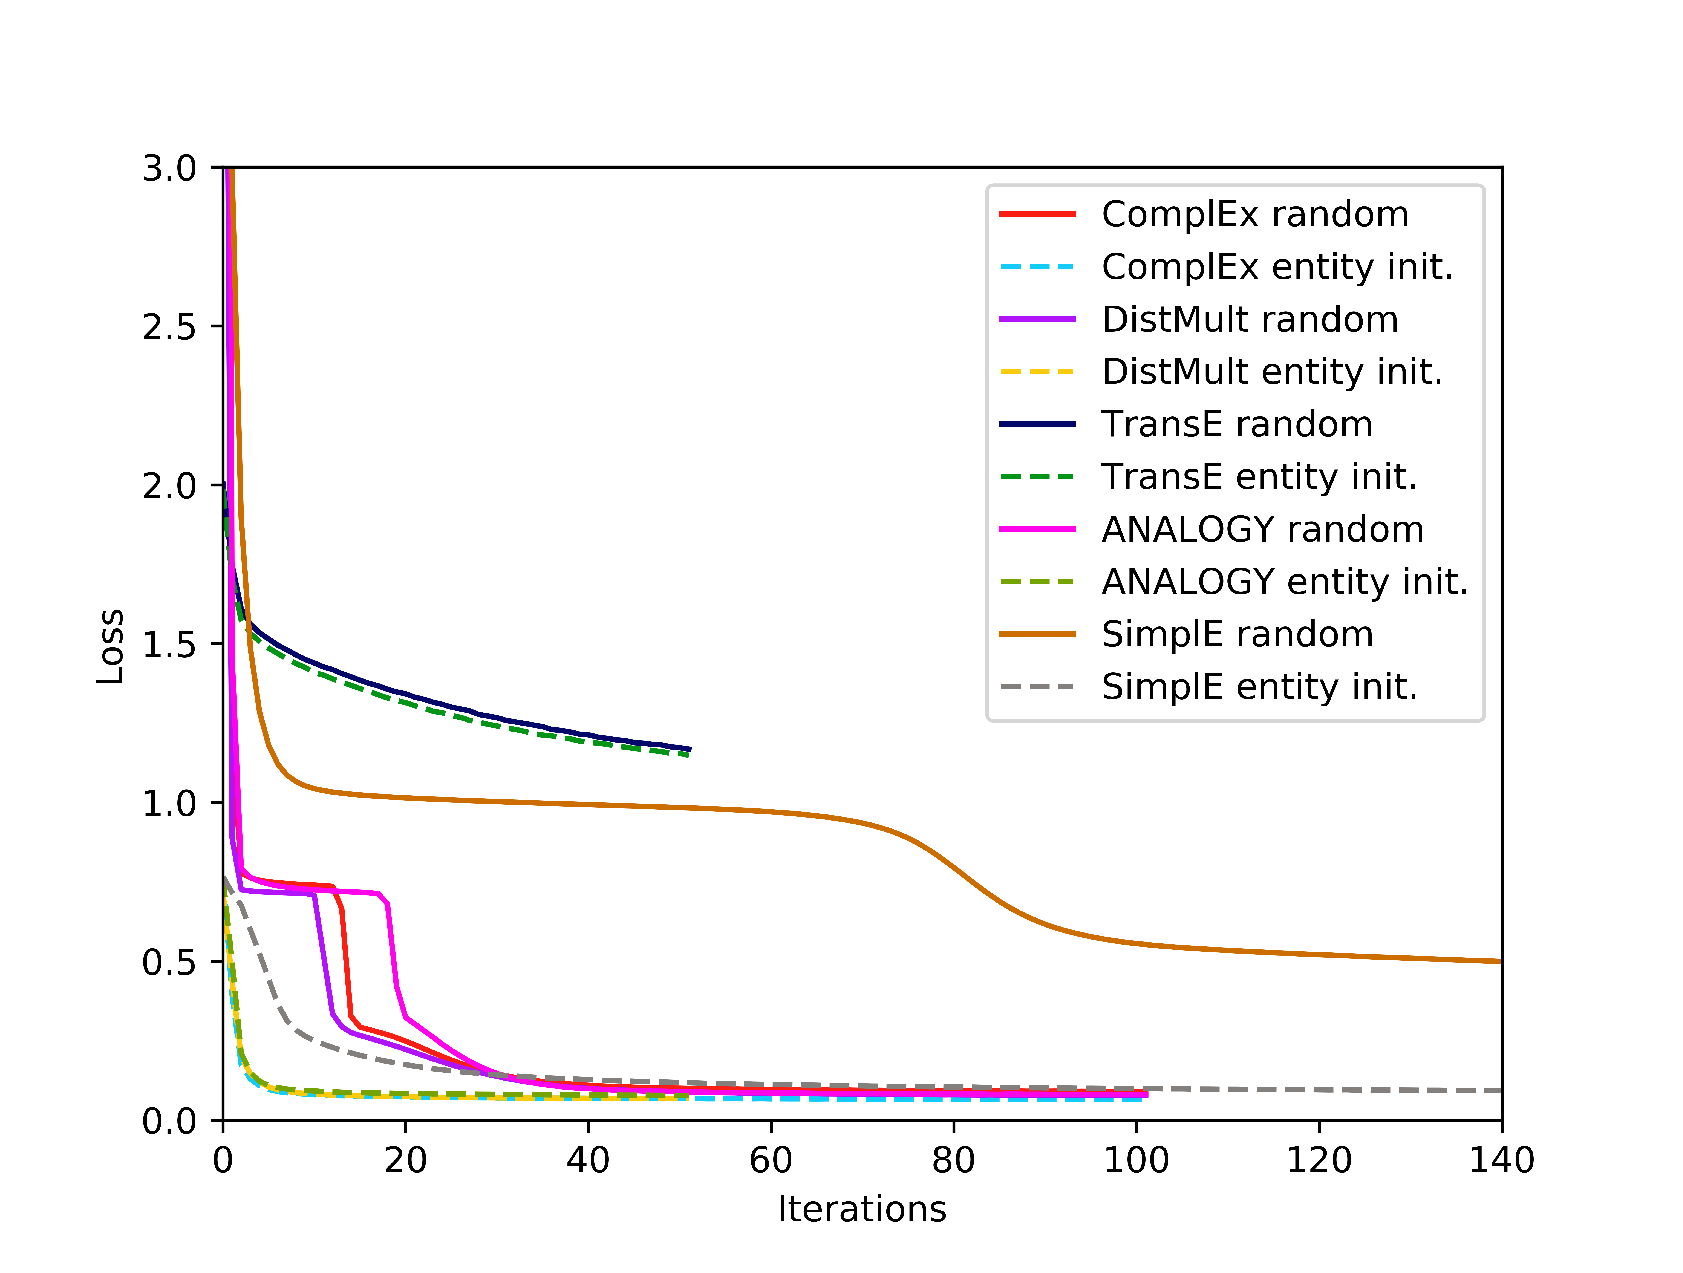
\includegraphics[width=.8\linewidth]{4_kbsintegrationdl/figures/ConvergenceDetail.eps}
    \caption{Loss convergence per iteration for each studied model according to the employed initialization. Dashed lines relate to entity initialization, whereas solid lines represent random initialization.}
    \label{fig:convergence}
\end{figure}


In TransE, no improvement is observed in neither of the studied datasets. This is directly related to the model's conception, as embeddings are generated following a geometrical approach, not considering latent semantics. Therefore, the additional semantic background provided by the initialization is not exploited by the model and is treated equally as randomly valued initialization.

Besides the improvement in terms of metrics, simple entity initialization has a direct benefit in the training of the KGE models, easing their convergence and reducing the number of iterations. Figure \ref{fig:convergence} evidences that simple entity initialization makes KGE models converge to a stable solution faster than those using random initialization. This statement does not hold in the case of TransE, since the convergence rate of both initialization options remains almost identical.

\subsubsection{Semantic-Based Initialization.}

\begin{figure}[t]
    \centering
    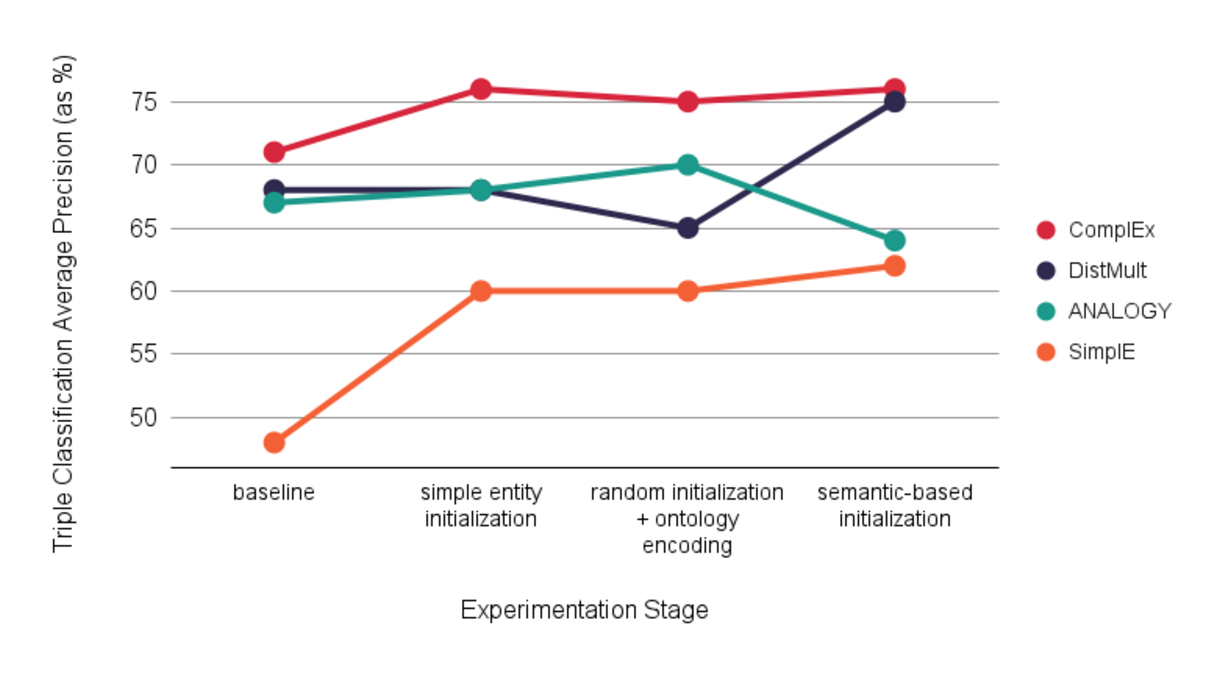
\includegraphics[width=.9\linewidth]{4_kbsintegrationdl/figures/WN_Comparison.eps}
    \caption{WN11 triple classification average precision (in percentage) per model and experimentation stage. Triangle, square, circle and star icons depict the results by ComplEx, DistMult, ANALOGY and SimplE, respectively. }
    \label{fig:wn_stage_comparison}
\end{figure}

According to the results reported in Table \ref{tab:exp_ont_intro}, the application of the complete semantic-based initialization induces an additional improvement over the results achieved with simple entity initialization. In WN11, the results of ComplEx, DistMult and SimplE employing semantic-based initialization noticeably outperform their corresponding baseline models. Figure \ref{fig:wn_stage_comparison} depicts the gradual improvement of each KGE model on WN11. In DistMult, the increment is particularly remarkable, where the baseline model reached a 68\% TCAP, but the introduction of ontological information alongside entity increases this value up to 75\%. The improvement in the case of SimplE is even more noticeable, where the baseline model achieved an accuracy of under 50\%. Semantic-based initialization increases the baseline value in about a 15\%, leading to a total of 62\%. This increment, although less pronounced, is also reflected in ComplEx results. Furthermore, the introduction of ontological information, even with random entity initialization, remarkably improves the baseline models' performance. The simplicity of the employed ontology, comprised of only four disjoint classes, plays a crucial role in this improvement. 

In FB13, although less noticeable, there is still an improvement in several of the reported KGE models. In this scenario, entity initialization does not further enhance the results introduced by adding ontological information to the random initialization. This may be related to the nature of each dataset, as WN11 models semantic relations between words, and can therefore benefit from the inclusion of explicit semantic information. Regarding the ontology choice, it can not be ascertained whether the complexity of the ontology directly impacts the results, as both ontologies produce similar results. Nonetheless, the complexity of the ontology could play a key role in the link prediction task, as it would significantly reduce the dimension of the candidate pool in tasks such as subject or object prediction.


\subsubsection{OOKB Entity Reasoning.}
Once proven that semantic-based initialization enhances the performance of KGE models, the extent of this proposal is evaluated over facts including OOKB entities. As evidenced by the results reported in Table \ref{tab:exp_entity_init}, initializing entities with word embeddings increases the specific knowledge about the entities, providing information that may not be inferred otherwise. Additionally, the inclusion of ontological information improves the generalization aspect of the model, enabling the inference of general restrictions about the relations, which directly translates into an accuracy improvement. Considering these two aspects, the fitness of semantic-based initialization for OOKB entity reasoning is evaluated (Table \ref{tab:OOKB_exp})

\begin{figure}[t!]
    \centering
    \subfigure[FB13 TCAP per relation \label{fig:fb13_tcap}]{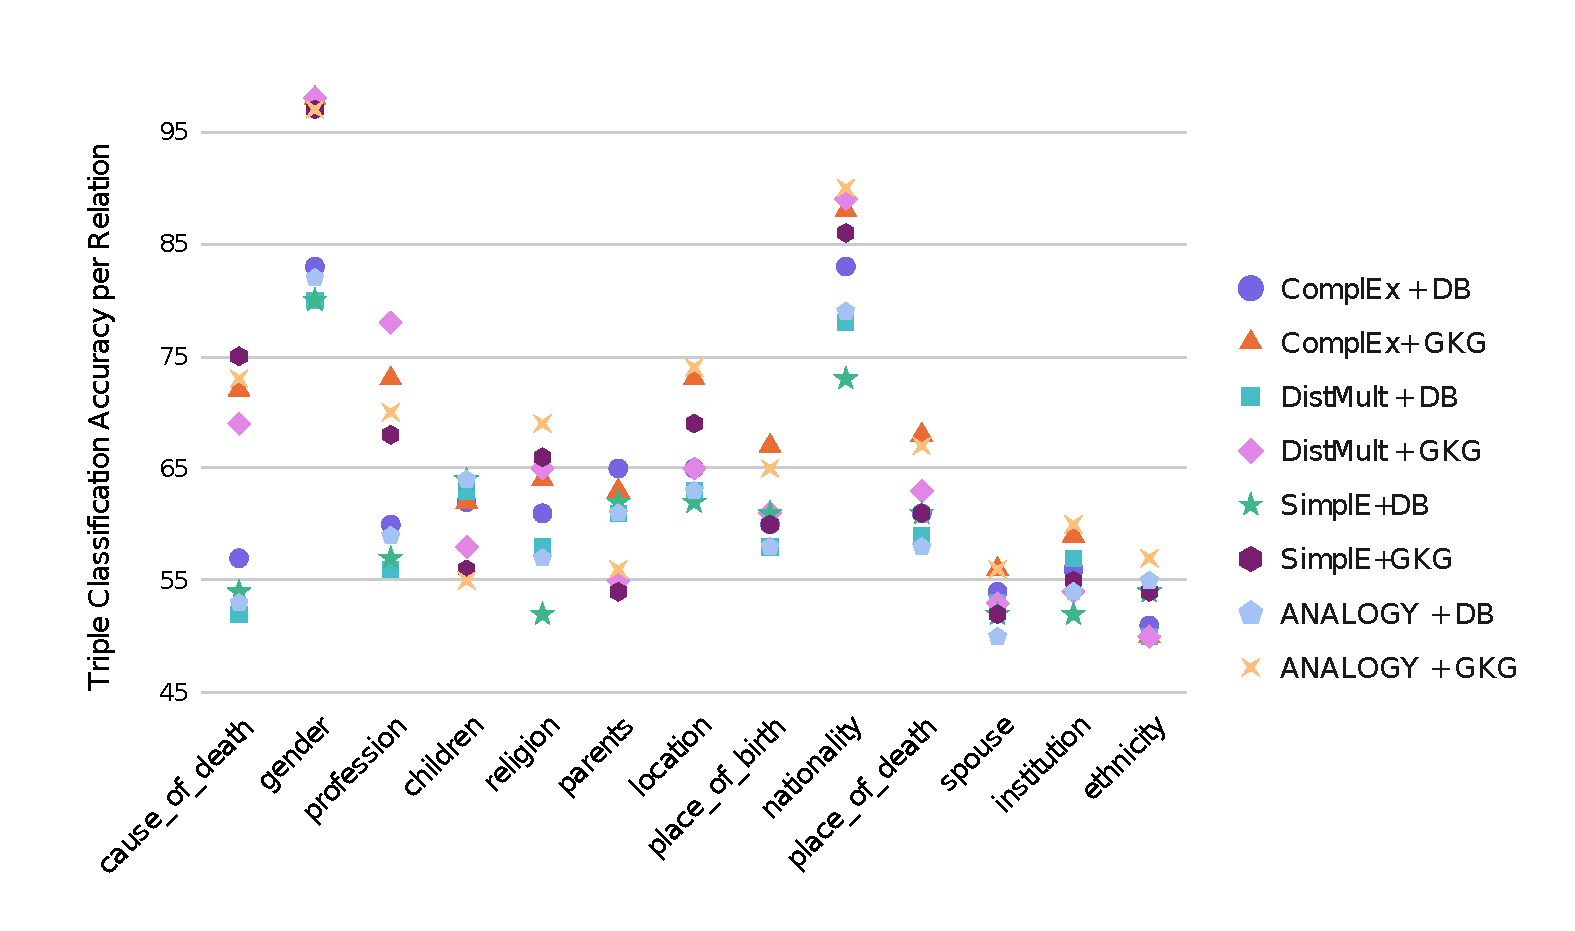
\includegraphics[width=.9\columnwidth]{4_kbsintegrationdl/figures/FB_relation_tcap.eps}}
    \subfigure[WN11 TCAP per relation \label{fig:wn11_tcap}]{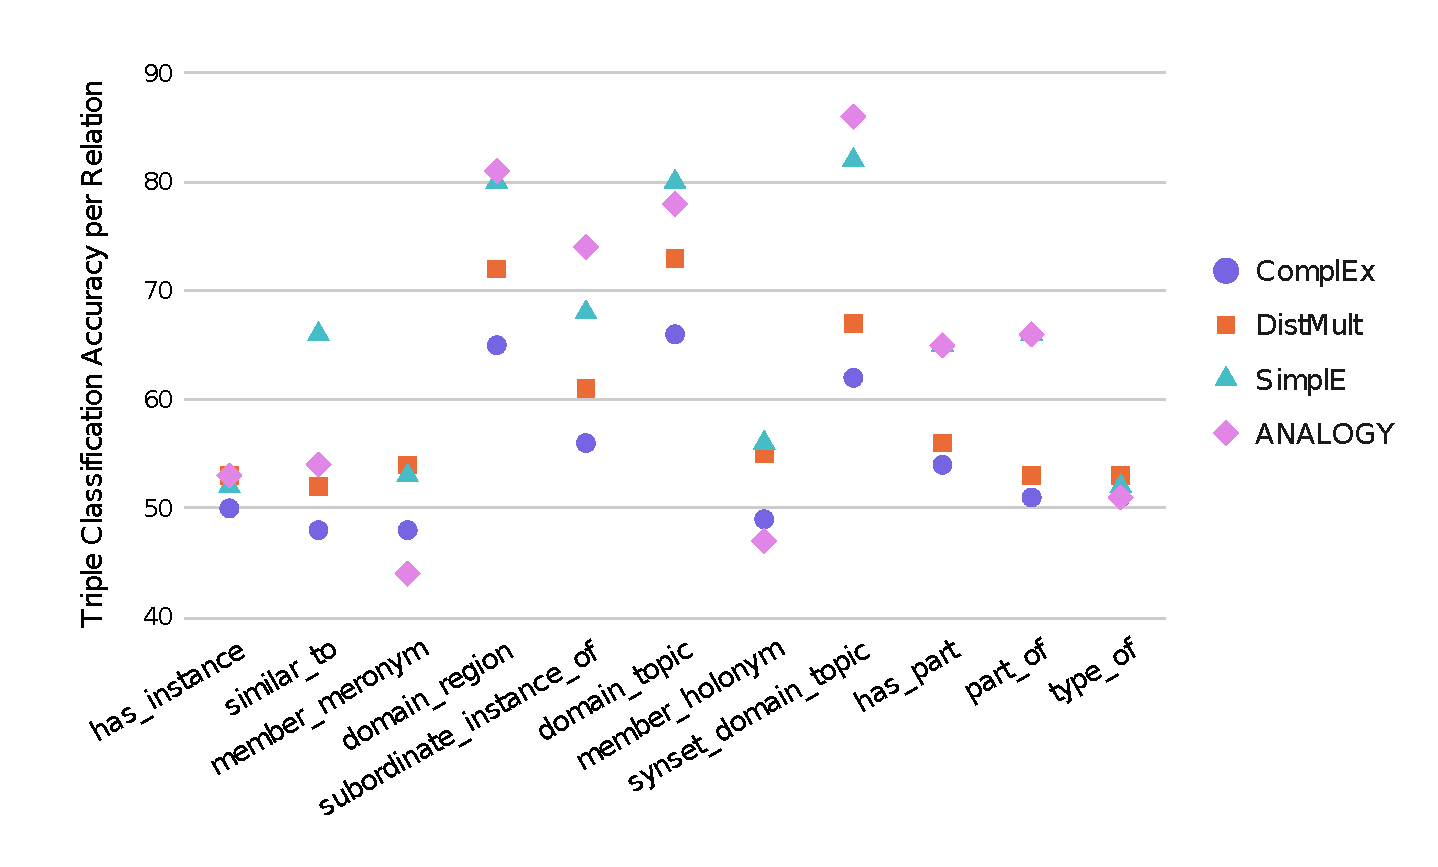
\includegraphics[width=.9\columnwidth]{4_kbsintegrationdl/figures/WN_relation_tcap.eps}}
    \caption{Triple classification average precision (TCAP) in percentage per relation on the OOKB datasets. Figure \ref{fig:fb13_tcap} provides the results on FB13, while Figure \ref{fig:wn11_tcap} illustrates the results obtained in WN11.}
    \label{fig:tcap_OOKB}
\end{figure}

In WN11, while semantic-based initialization considerably enhances the models' performance, no strict class restrictions can be inferred due to the simplicity of the ontology. Therefore, even though the models achieve a high precision over the fully-known test set, this attainment is not extended to the OOKB test set, where the TCAP barely exceeds 50\%. Figure \ref{fig:wn11_tcap} provides an insight on the results obtained by each model on the OOKB test set on each relation. As showcased in the Figure, although the TCAP value ranges between 50\% and 60\% in most relations, it rises to around 70\% in relations such as \textit{domain region} and \textit{domain topic}.

Table \ref{tab:ookb_fb} shows that the results achieved in FB13 for the OOKB test set are similar to those obtained for the fully-known test set, except for DistMult. This phenomenon is related to the type of information modelled in FB13, as the restrictions associated with the relations are closely related to the classes of entities. This statement is further validated by the results in Figure \ref{fig:fb13_tcap}, where the average precision in half of the studied relations reaches more than 70\%. These results show a direct correlation between the homogeneity of the subject and object classes of the relation and the TCAP obtained. Therefore, in relations such as \textit{children}, \textit{parents} or \textit{spouse} that always relate two entities of type \textit{Person}, the precision is always close to 60\% as restrictions are easily inferred. Similarly, the relations \textit{location} and \textit{nationality} also achieve a remarkable performance in terms of precision, even though the results fluctuate across the different models. In both relations, the models employing the GKG ontology achieve better results than those using the DBpedia ontology. This is a direct consequence of the fine-graining level provided by the DBpedia ontology for the general class \textit{Place}, where more than 170 subclasses are identified.

\subsubsection{Performance Analysis.}
%%AQUI VA LO DEL PERFORMANCE ANALYSIS COMO SU NOMBRE INDICA
In addition to improving the transferability, OOKB reasoning via semantic-based initialization can be used to assess the robustness of the KGE model. After evaluating the semantically initialized model on both the fully-known and the OOKB test set, their metrics can be compared. Being $TCAP_{FK}$ and $TCAP_{OOKB}$ the TCAP values of the fully-known and OOKB test sets, respectively, three scenarios can be identified:
\begin{itemize}
    \item \textit{$TCAP_{FK} \gg TCAP_{OOKB}$:} A disparity in favour of the fully-known set can indicate an inapt introduction of ontological information. This induces an exploitative training approach to the KGE model, where the predictions are mainly based on the particularities of the entities. The imbalance in the results may be related to the type of ontological information employed, as well as its complexity. If the KG coverage of the selected ontological information is minimal (i.e., too many rules are selected, or the class hierarchy is too complex), then this can potentially cause a flaw. Simpler ontological information, or a different encoding approach, could solve this imbalance and enhance the generalization capacity of the model. This would result in an improvement of the models' coverage, as well as enabling information sharing between existing and upcoming entities.
    
    \item \textit{$TCAP_{FK} \approx TCAP_{OOKB}$:} A similarity in the results achieved by both sets indicates that the model is appropriately including the ontological information. In this scenario, the KGE model is inferring accurate restrictions about relations, enabling the coverage of OOKB entities. A slight difference in the metrics favouring the fully-known set is expected.
    
    \item \textit{$TCAP_{FK} \ll TCAP_{OOKB}$:} A non-optimal parameter selection can result in an imbalance in favour of the OOKB set. Insufficient learning of specific entity knowledge can result in this result mismatch, indicating that the model has not converged to its optimal solution, but diverged.
\end{itemize}

\subsection{Design Compliance}\label{4_sec:method_assessment}
\begin{figure}[ht]
    \centering
    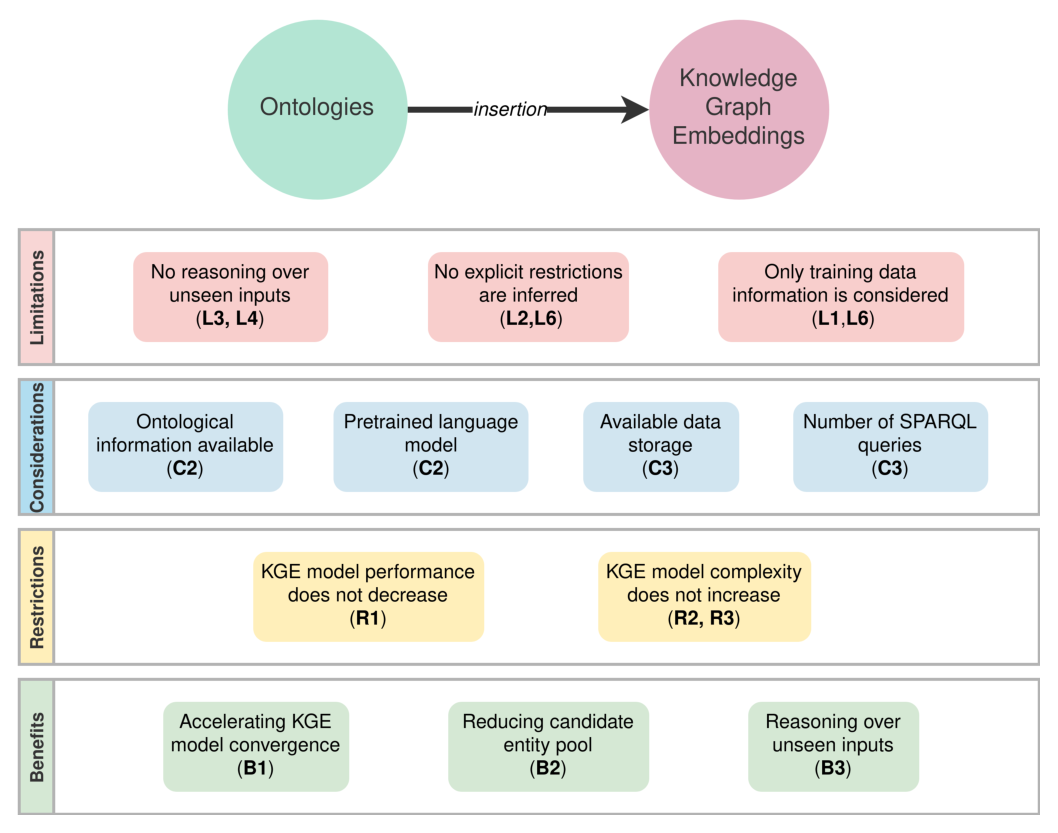
\includegraphics[width=\linewidth]{4_kbsintegrationdl/figures/Instance_KB_into_DL.eps}
    \caption{Method overview on the introduction of ontologies into knowledge graph embedding models. In bold, the general method parameters as depicted in Figure \ref{fig:overview_kbs_dl_intro}.}
    \label{fig:instance_method_kbs_into_dl}
\end{figure}

Semantic-based initialization instantiates the introductory integration method proposed in Section \ref{4_sec:methodology_kbs_intro_dl}. Figure \ref{fig:instance_method_kbs_into_dl} depicts the specific integration parameters of the presented case:

\paragraph{Limitations}
\begin{itemize}
    \item \textbf{No reasoning over unseen inputs.} One of the main challenges regarding KGE models is the codification of unseen elements. KGE models generate representations for the elements existing in a KG during the training time. After training, the representations of each entity and relations are stored in a keyed structure. Hence, if the model is queried for the representation of an unseen element, no representation can be returned as it has no key assigned. Retraining the model from scratch is then needed to generate a feasible representation for unseen elements, limiting its transferability (\ref{kbsintrodl_L_transfer}). While the approaches presented in Section \ref{4_sec:ontointro_kgc} potentially solve this issue, they still require at least a partial retraining. Therefore, the benefit of generating a representation for a single element is severely imbalanced with respect to its computational cost (\ref{kbsintrodl_L_cost}). 
    
    \item \textbf{No explicit restrictions are inferred.} KGE models follow an exploitative training approach. Therefore, the restrictions learned about facts are only based on the training data, which can be subject to errors and lead to inconsistencies (\ref{kbsintrodl_L_constraint}). The constraints learned by the KGE model can therefore be inaccurate and produce different outputs for seemingly similar entities (\ref{kbsintrodl_L_brittleness}).  
    
    \item \textbf{Only training data information is considered.} While there are approaches that extend KGE models with external information, baseline KGE models only consider training data for embedding generation. Using training data as the only source bounds the embeddings to the quality and quantity of the data (\ref{kbsintrodl_L_data_hungry}). Including external data sources could ease the reliance of the model on the training data, as well as potentially enabling the inference of better internal patterns (\ref{kbsintrodl_L_constraint}). 
\end{itemize}
\paragraph{Considerations}
\begin{itemize}
    \item \textbf{Ontological information available.} Ontologies play a fundational role in the generation of KGs, serving as a scaffold for the introduction of new elements. Even though the KG and the ontology are closely related, they may not be always disclosed together. Therefore, while the KG may be publicly available, its ontological information may remain unveiled (\ref{kbsintrodl_C_data}) or may only be accessible via queries.
    
    \item \textbf{Pretrained language model.} The proposed initialization replaces random values with meaningful semantic representations. A pretrained language model is used to generate the initial representations. There is a wide variety of existing models, each trained on their specific corpus and with different embedding dimensions. The selected language model should be aligned with the nature of the knowledge contained in the KG, as well as providing representations of a dimension compatible with the KGE (\ref{kbsintrodl_C_data}).
    
    \item \textbf{Available data storage.} Semantic-based initialization does not require any additional processing resources, such as GPU units. However, it can cause a higher demand on the storage capacity, as it requires the storage of information external to the KG. The data required for initialization is not as sizable at the KG itself, but it is still necessary to ensure that there is enough capacity for its storage (\ref{kbsintrodl_C_resource}).
    
    \item \textbf{Number of SPARQL queries.} In those cases where the ontology files are not available, a SPARQL endpoint may be used to retrieve the required information. For each targeted element in the graph (entities or relations), a SPARQL query may be set to retrieve the specific ontological information. Subsequently, the number of queries grows linearly with the size of the KG. While SPARQL queries have execution times of fractions of a second, if the number of queries to execute is elevated, it can translate into high execution times. Additional, as SPARQL queries are performed online, they are subjected to latency and network failures (\ref{kbsintrodl_C_resource}). 
\end{itemize}
\paragraph{Restrictions}
\begin{itemize}
    \item \textbf{KGE model performance must not decrease.} One of the general restrictions of the proposed method, \ref{kbsintrodl_R_performance} states that to perform KBS introduction, it must be ensured that the performance of the primary DL model will not decrease. This restriction is satisfied in the proposed use case, as none of the studied KGE models experience a decrement on its performance metrics. 
    
    \item \textbf{KGE model complexity does not increase.} The KGE models studied in this use case all have a complexity order of $\mathcal{O}(d)$, where $d$ is the dimension of the embeddings. However, this is  not the case for every KGE model. In Graph Neural Networks, their complexity order is not related to the dimension of the embedding, but to the number of entities and relations in the graph, which can lead to considerably more complex models. Semantic-based initialization is performed offline, thus ensuring that the complexity of the model remains unchanged (\ref{kbsintrodl_R_complexity}). Moreover, as it is performed independently from the KGE model, it does not increase the required training resources (\ref{kbsintrodl_R_resource}).
\end{itemize}
\paragraph{Benefits}
\begin{itemize}
    \item \textbf{Accelerating KGE model convergence.} Figure \ref{fig:convergence} depicts the learning curves of the considered KGE models with and without semantic-based initialization. Even though each pair of models (initialized and non-initialized) are trained for the number of epochs, the difference in their convergence rate is visibly noticeable. Non-initialized models present dramatic changes in the shape of their learning curves, reaching their final inflection point considerably later than their initialized counterparts. The presented use case therefore showcases the fulfilment of benefit \ref{kbsintrodl_B_convergence}.
    
    \item \textbf{Reducing candidate entity pool.} In link prediction, the goal is to find the missing entity of an incomplete fact such that its feasibility is maximized. In the case of subject prediction, given an incomplete fact $(?,p,o)$, each potential fact $(e,p,o)$ $\forall e \in \mathcal{E}$ is computed and rated in decreasing order. The element featured in the top position is outputted by the model as the solution. If explicit restrictions about the subject and object elements featured on each predicate are included in the model, the pool of candidate entities is reduced to those entities in $\mathcal{E}$ that fit the restriction of the relation. Therefore, the computation of feasible triples is reduced to $(e,p,o)$ $\forall e \in \mathcal{E}'$, being $\mathcal{E}'$ the set of entities that fit the relation constraints. This reduces the computation time of the model, which subsequently benefits from the introduction of explicit constraints (\ref{kbsintrodl_B_restrictions}).
    
    \item \textbf{Reasoning over unseen inputs.} One of the main outcomes of the proposed initialization is the induced capacity of KGE models to reason over unseen inputs. Semantic-based initialization enables a descriptive and unique representation of unseen elements without the need of explicitly declaring additional facts or knowledge about them (\ref{kbsintrodl_B_reduce}). However, the level of inference enabled over unseen elements remains superficial and therefore should not be used to directly introduce new facts into the KG. Instead, it can be treated as a filtering element to find potential introduction candidates.
\end{itemize}


\section{Summary}\label{4_sec:summary}
This chapter addresses two of the contributions of this thesis: \textbf{C1} and \textbf{C4}. Section \ref{4_sec:methodology_kbs_intro_dl} outlines contribution \textbf{C1: design method for the insertion of knowledge-based systems into deep learning models}. This method addresses the existing limitations within DL models from an introduction perspective (e.g., brittleness, lack of constraint enforcement, or limited transferability), providing also prior considerations and restrictions that should be met for the integration to be successful, such as stable model performance and model complexity. The general benefits derived from the integration are also depicted. Moreover, this contribution also supports the attainment of objective \textbf{O1: define a set of general parameters per dimension for each integration of knowledge-based systems and deep learning models}. 

Knowledge graph completion provides a fitting scenario for the application of the design method depicted in C1, following the achievement of objective \textbf{O2: instantiate the proposed design method across different models and use scenarios}. Knowledge graph embedding (KGE) models, which are based on deep learning, are the predominant paradigm in this area, presenting two main shortcomings that can be resolved with the introduction of KBS: i) lack of background information, ii) inability to reason over inputs that are not present during training (out-of-knowledge-base entities). A semantic initialization method based on ontologies is proposed to deal with the aforementioned shortcomings. The proposed initialization is another contribution of this thesis, \textbf{C4: semantic-based initialization method for knowledge graph embedding models}. The encoding of ontological information within the KGE model improves the results achieved by the baseline models while considerably accelerating their convergence. Moreover, it also enables reasoning over unseen elements of the graph, addressing one of the main open challenges in the context of knowledge graph completion. 

The compliance of the proposed initialization is then assessed with respect to the general design method, fulfilling the objective \textbf{O3: assessing the compliance of each implementation with respect to the general design parameters}. 